\chapter{Verification of Deep Learning}\label{chap:verificationchap}

Successful experience from industrial software engineering, which produced software that is currently applied in safety-critical applications, such as automotive and avionic applications, suggests that, to develop high-quality and low-cost software in a limited production time, a software development life cycle (SDLC) process is required. As illustrated in Figure~\ref{fig:oldVmodel} about a V-model for SDLC, verification is a key process throughout the development lifecycle.   This chapter will discuss a specific verification task, i.e., given a trained machine learning model and a robustness property, it is to determine whether the robustness property holds on the model. After the definition of robustness property in Section~\ref{sec:robusntessproperty}, we will present representative examples for two categories of verification algorithms in Section~\ref{chap:MILP} and Section~\ref{chap:reachabilityAnalysis}, respectively. 
%
\begin{figure}[!htbp]
    \centering
    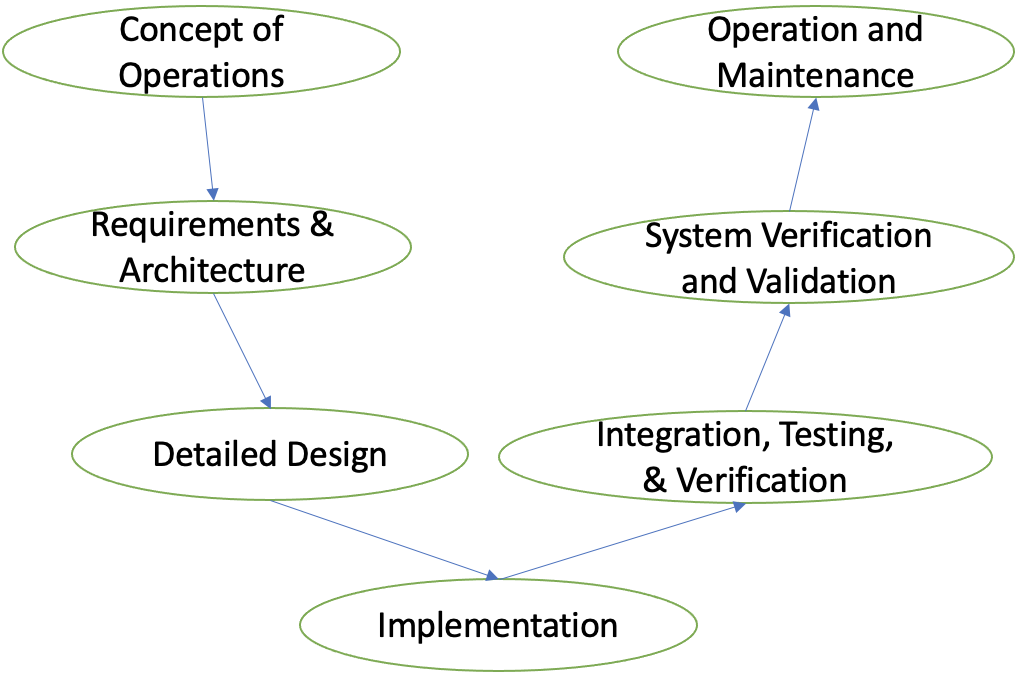
\includegraphics[width=0.6\textwidth]{images/robustnessVerification/oldVmodel.png}
    \caption{An illustrative V-model for software development}
    \label{fig:oldVmodel}
\end{figure}
%


%
Existing verification algorithms can be roughly categorised into exhaustive search \cite{HKWW2017}, constraint-solving based methods~%
%such as
\cite{katz2017reluplex}, abstract interpretation based methods~%
%such as
\cite{gehr2018ai,10.1007/978-3-030-32304-2_15},  global optimisation \cite{ruan2018global,RWSHKK2018}, game-based methods~\cite{wicker2018feature,wu2018game}, and symbolic interval analysis \cite{10.1007/978-3-030-32304-2_15,10.1145/3368089.3417918,10.1007/s00165-021-00548-1}. The readers are referred to \cite{HUANG2020100270} for a survey. 
%These methods ensure  the completeness and the soundness of the results. 
Moreover, in addition to the pixel perturbations measured with norm distances, we are also looking into real-world perturbations such as geometric and spatial perturbations \cite{GeoRobust2022}.  
%
This chapter presents a few typical verification algorithms. The first algorithm of this chapter (Section~\ref{chap:MILP}) reduces the verification to a constraint solving problem, which can then be solved with an off-the-shelf solver. The algorithm is white-box, and the reduction needs to consider the internal architecture of the neural networks. The complexity is NP-complete with respect to the combined number of hidden neurons and input features. 
%
On the other hand, the second algorithm (Section~\ref{chap:reachabilityAnalysis}), as some others  \cite{ruan2018global,RWSHKK2018,wicker2018feature,wu2018game,GeoRobust2022}, is black-box, i.e., they do not rely on the internal architecture of the neural networks. Theoretically, this brings a significant advantage that the computational complexity of the verification problem is NP-complete with respect to the number of input features. While the complexity class does not change, the number of hidden neurons can be an unlimited number of times more than that of input features, due to the current trend of deep learning on training deeper and larger networks. Also, black-box verification means that we can work with neural networks of any scale and structure. 

\section{Robustness Properties for Verification}\label{sec:robusntessproperty}

A (deep and feedforward) neural network, or neural network, can be defined as a tuple $\network=(\layers,
\layerConnections, \Phi)$, where $\layers=\{\layers_k~|~k\in\{1..K\}\}$ is a set of layers,
$\layerConnections\subseteq \layers\times \layers$ is a set of connections between layers and 
$\Phi=\{\phi_k~|~k\in\{2..K\}\}$ is a set of functions, one for each non-input layer.
%
%between layers
%$f_k:D_{L_{k-1}}\rightarrow D_{L_k}$ such that $D_{L_{k}}$ is the vector space of layer $k$. 
%
In a neural network, $\layers_1$ is the \emph{input} layer, $\layers_{K}$ is the \emph{output} layer,
and layers other than input and output layers are called \emph{hidden layers}.
Each layer $\layers_k$ consists of $s_k$ %nodes, which are also called
\emph{neurons} (or nodes).
The $l$-th node of layer $k$ is denoted by $n_{k,l}$.


Each node $n_{k,l}$ for $2 \leq k\leq K$ and  $1\leq l\leq s_k$ is associated with two variables $u_{k,l}$ and $v_{k,l}$, to record  its values before and after an activation function, respectively.
%
The Rectified Linear Unit (ReLU) \cite{relu} is one of the most popular 
%and effective 
activation functions for neural networks, according to which the \emph{activation 
value} of each node of hidden layers is defined as
%
\begin{equation}
    \label{eq:relu}
    v_{k,l}=ReLU(u_{k,l})=
    \begin{cases}
        u_{k,l} &\mbox{  if } u_{k,l}\geq 0 \\
            0 & \mbox{  otherwise}
    \end{cases}
\end{equation}
%\james{Definition (3) seems to put $u$ and $v$ as output and input - rather than as used in (2) as input and output respectively. Have I missed something here?}\xiaowei{it's ok}

%
Each input node $n_{1,l}$ for $1\leq l\leq s_1$ is associated with a
variable $v_{1,l}$ and each output node $n_{K,l}$ for $1\leq l\leq s_K$ is
associated with a variable $u_{K,l}$, because no activation function is
applied on them. Other popular activation functions beside ReLU include: Sigmoid, Tanh, and Softmax. 

% We use $u_{k,l}$ to denote
%the value of $n_{k,l}$. 
Except for the nodes at the input layer, every node is connected to nodes in the
preceding layer by pre-trained parameters such that for all $k$ and $l$ with
$2 \leq k\leq K$ and  $1\leq l\leq s_k$
%
\begin{equation}
  \label{eq:sum}
  u_{k,l}=b_{k,l}+\sum_{1\leq h \leq s_{k-1}} w_{k-1, h, l}\cdot v_{k-1,h}
\end{equation}
%
where $w_{k-1,h,l}$ is the weight for the connection between
$n_{k-1,h}$ (i.e., the $h$-th node of layer $k-1$) and $n_{k,l}$
(i.e., the $l$-th node of layer $k$), and $b_{k,l}$ the
so-called \emph{bias} for node $n_{k,l}$.  We note that this
definition can express both fully-connected functions and
convolutional functions\footnote{Many of the surveyed techniques can work with other types of functional layers such as max-pooling, batch-normalisation, etc. Here  for simplicity, we omit their expressions.}.
%
The function $\phi_k$ is the composition of Equation (\ref{eq:relu}) and (\ref{eq:sum}) by having $u_{k,l}$ for $1\leq l\leq s_k$ as the intermediate variables. Owing to the use of the ReLU as in \eqref{eq:relu}, the behavior of a neural
network is highly non-linear. 

Let $\real$ be the set of real numbers. We let $\mathcal{D}_{k} = \real^{s_k}$ be the vector space
associated with layer $\layers_k$, one dimension for each variable $v_{k,l}$. 
Notably, every point $\textbf{x}\in \mathcal{D}_{1}$ is an input. Without loss of generality, the dimensions of an input are normalised as real values in $[0,1]$, i.e., $\mathcal{D}_1=[0,1]^{s_1}$. 
%Moreover, we let $n=s_1$ and $m=s_K$.
%
A neural network $\network$ can alternatively be expressed as a function $f: \mathcal{D}_{1}\rightarrow \mathcal{D}_{K}$ such that 
\begin{equation}
f(\textbf{x}) = \phi_{K}(\phi_{K-1}(...\phi_2(\textbf{x})))
\end{equation}
%
Finally, for any input, the neural network $\network$ assigns a \emph{label}, that is,
the index of the node of output layer with the largest value:
\begin{equation}
\mathit{label}=\mathrm{argmax}_{1\leq l\leq s_K}u_{K,l}
\end{equation}
Moreover, we let $\C=\{1..s_K\}$ be the set of labels. 
\begin{example}
Figure \ref{fig:nn} is a simple neural network with four layers. 
The input space is $\mathcal{D}_{1}=[0,1]^2$, the two hidden vector spaces are $\mathcal{D}_2=\mathcal{D}_3=\real^3$, and the set of labels is $\C=\{1,2\}$.

\begin{figure}[htp!]
\centering

\def\layersep{1.8cm}

\scalebox{1}{
\begin{tikzpicture}[shorten >=1pt,->,draw=black!50, node distance=\layersep]
    \tikzstyle{every pin edge}=[<-,shorten <=1pt]
    \tikzstyle{neuron}=[circle,fill=black!25,minimum size=15pt,inner sep=0pt]
    \tikzstyle{input neuron}=[neuron, fill=green!50];
    \tikzstyle{output neuron}=[neuron, fill=red!50];
    \tikzstyle{hidden neuron}=[neuron, fill=blue!50];
    \tikzstyle{annot} = [text width=4em, text centered]

    % Draw the input layer nodes
    \foreach \name / \y in {1,...,2}
    % This is the same as writing \foreach \name / \y in {1/1,2/2,3/3,4/4}
        \node[input neuron, pin=left:$v_{1,\y}$] (I-\name) at (0,-\y) {};
        %\node[input neuron, pin=left:Input \#\y] (I-\name) at (0,-\y) {};

    % Draw the 1st hidden layer nodes
    \foreach \name / \y in {1,...,3}
        \path[yshift=0.5cm]
            node[hidden neuron] (H1-\name) at (\layersep,-\y cm) {};

    % Draw the 2nd hidden layer nodes
    \foreach \name / \y in {1,...,3}
        \path[yshift=0.5cm]
            node[hidden neuron] (H2-\name) at (\layersep*2,-\y cm) {};

    % Draw the output layer node
    \node[output neuron,pin={[pin edge={->}]right:$v_{4,1}$}, right of=H2-2, yshift=0.5cm] (O1) {};
    \node[output neuron,pin={[pin edge={->}]right:$v_{4,2}$}, right of=H2-2, yshift=-0.5cm] (O2) {};

    % Connect every node in the input layer with every node in the
    % hidden layer.
    \foreach \source in {1,...,2}
        \foreach \dest in {1,...,3}
            \path (I-\source) edge (H1-\dest);

    \foreach \source in {1,...,3}
        \foreach \dest in {1,...,3}
            \path (H1-\source) edge (H2-\dest);

    \foreach \source in {1,...,3}
         \path (H2-\source) edge (O1);

    \foreach \source in {1,...,3}
         \path (H2-\source) edge (O2);

    % Annotate the layers
    \node[annot,above of=H1-1, node distance=1cm] (hl1) {Hidden layer};
    \node[annot,above of=H2-1, node distance=1cm] (hl2) {Hidden layer};
    \node[annot,left of=hl1] {Input layer};
    \node[annot,right of=hl2] {Output layer};

    \node[annot, right of=H1-1, node distance=0.0cm] (hl1) {\small $n_{2,1}$};
    \node[annot, right of=H1-2, node distance=0.0cm] (hl1) {\small $n_{2,2}$};
    \node[annot, right of=H1-3, node distance=0.0cm] (hl1) {\small $n_{2,3}$};
    \node[annot, right of=H2-1, node distance=0.0cm] (hl1) {\small $n_{3,1}$};
    \node[annot, right of=H2-2, node distance=0.0cm] (hl1) {\small $n_{3,2}$};
    \node[annot, right of=H2-3, node distance=0.0cm] (hl1) {\small $n_{3,3}$};
\end{tikzpicture}
}
  \caption{A simple neural network}
  \label{fig:nn}
\end{figure}

\end{example}
\bigskip

%\paragraph{Neural network instance}

Given one particular input $\textbf{x}$, the neural network $\network$ is
\emph{instantiated} and we use $\network[\textbf{x}]$ to denote this instance of the
network. In $\network[\textbf{x}]$, for each node $n_{k,l}$, the values of the variables $u_{k,l}$ and $v_{k,l}$ are fixed and denoted as $u_{k,l}[\textbf{x}]$ and $v_{k,l}[\textbf{x}]$, respectively. 
%of  of
%
Thus, the activation or deactivation of each ReLU operation in the network is similarly determined.  
%We
%write $u_{k,l}[\textbf{x}]$ for the value before applying the ReLU and $v_{k,l}[\textbf{x}]$
%for the value after applying the ReLU. 
We define
%
  \begin{equation}
    \label{eq:sign}
    \mathit{sign}_\network(n_{k,l},\textbf{x})=
    \begin{cases}
      +1 &\mbox{  if } u_{k,l}[\textbf{x}] = v_{k,l}[\textbf{x}] \\
      -1 & \mbox{  otherwise}
    \end{cases}
  \end{equation}
 %
The subscript $\network$ will be omitted when clear from the context. 
The classification label of $x$ is denoted as $\network[\textbf{x}].\mathit{label}$.

\begin{example}\label{example:weights}
%
Let $\network$ be a neural network whose architecture is given in Figure \ref{fig:nn}.  
Assume that the weights for the first three layers are as follows:
%   
$$
\textbf{W}_{1}={
\begin{bmatrix}
  4 & 0 & -1\\
  1 & -2 & 1
\end{bmatrix}},\,\,
\textbf{~~~W}_{2}={
\begin{bmatrix}
  2 & 3 & -1\\
  -7 & 6 & 4 \\
  1 & -5 & 9
\end{bmatrix}}
$$
and that all biases are 0. When given an input 
$\textbf{x}=[0, 1]$, we get $\mathit{sign}(n_{2,1},\textbf{x})=+1$, since
$u_{2,1}[\textbf{x}]=v_{2,1}[\textbf{x}]=1$, and $\mathit{sign}(n_{2,2},\textbf{x})=-1$,
since $u_{2,2}[\textbf{x}] = -2 \neq 0 = v_{2,2}[\textbf{x}]$. 
%
\end{example}


\subsection*{Robustness as an Optimisation Problem}

We have defined robustness in Section~\ref{sec:adversarialexample}. For robustness verification, given an input $\textbf{x}$, a $d$-neighbourhood $\eta(\textbf{x},L_p,d)$ (as in Definition~\ref{def:inputregion}), and a neural network $f$, it is to check whether all inputs within the $d$-neighbourhood have the same label, i.e., 
\begin{equation}\label{equ:verification1}
    \forall \textbf{x}': ||\textbf{x}-\textbf{x}'||_p < d \Rightarrow \hat{f}(\textbf{x}) = \hat{f}(\textbf{x}')
\end{equation}
where $\hat{f}(\textbf{x})$ returns the predictive label of $\textbf{x}$ by $f$. Alternatively, this can be reduced to first finding the maximum safety radius $\delta$ such that
\begin{equation}\label{equ:verification}
    \begin{array}{rl}
     \displaystyle \delta \defequal  \min_{\textbf{x}'}   &  ||\textbf{x} - \textbf{x}'||_p \\
       s.t.  & \hat{f}(\textbf{x}) \neq \hat{f}(\textbf{x}') \\
    \end{array}
\end{equation}
Then, it is to check whether $d\leq \delta$ as the verification result. 



\section{Reduction to Mixed Integer Linear Programming (MILP)}\label{chap:MILP}

In this chapter, we present how we can reduce the verification problem (Equation (\ref{equ:verification})) to the mixed integer linear programming (MILP) problems, so that it can be solved with the off-the-shelf MILP solvers. We will also consider the over-approximation of the problem so that it is able to be solved with linear programming. We will focus on the ReLU neural network (i.e., all activation functions are ReLU) and the robustness property.

\subsection{Reduction to MILP}

Let $\textbf{x}_c$ be the original input whose label is $y_c=\hat{f}(\textbf{x}_c)$. Recall from Chapter~\ref{sec:robusntessproperty} that, we assume the network $f$ has $K$ layers. Then, Equation (\ref{equ:verification}) can be rewritten as 
\begin{equation}\label{equ:robustnessreduction}
\begin{array}{rll}
  \displaystyle\max_{\textbf{x}}  &   ||\textbf{x} - \textbf{x}_c||_p & \\
    s.t. &  \textbf{x} = \textbf{v}_1, & \\
    & \textbf{up}_{i+1} =  \textbf{W}_i \vec{v}_{i} + \vec{b}_i, & i = 1..K-1\\
    & \textbf{v}_{i+1} = ReLU(\textbf{up}_{i+1}),  & i = 1..K-2 \\
    &  \textbf{up}_{K}(y_c) - \textbf{up}_{K}(y)\geq 0,  & y\in C \\
\end{array}
\end{equation}
where $\textbf{up}_{i},\textbf{v}_{i}$ denote the activation vector of layer $i$ before and after the ReLU function, respectively. 
The first condition confirms to have $\textbf{x}$ as the activation vector of the input layer. 
The second and third conditions implement the linear transformation and ReLU activation function of layer $i+1$, respectively. The fourth condition requires that $\textbf{x}$ has the label $y_c$.  Specifically, the label is $y_c$ if and and only if $\forall {y\in C}:  \textbf{up}_{K}(y_c) - \textbf{up}_{K}(y)\geq 0$. 


%Therefore, if Equation (\ref{equ:robustnessreduction}) returns a value $p^*\geq 0$ then we can conclude that the network $f$ is robust in the neighbourhood $\eta(\textbf{x}_c,L_p,d)$. 

Considering that the ReLU function is non-linear, we introduce two methods of transforming the second and third conditions of Equation (\ref{equ:robustnessreduction}) into MILP constraints, i.e., linear constraints with Boolean variables. 

\subsection*{Method One for Layers}

The first method requires one Binary variable for each neuron. Let $\vec{t}_{i+1}$ have value $0$ or $1$ in its entries and have the same dimension as $\vec{v}_{i+1}$, and $M$ be a very large constant number that can be treated as $\infty$. We do not need $\vec{u}_{i+1}$. Specifically, we have 
the following MILP constraints for every layer $i=1..K-2$ to replace the second and third conditions of Equation (\ref{equ:robustnessreduction}): 
%\begin{align*}
\begin{equation}\label{equ:MILPmethodone}
    \begin{array}{ll}
    \vec{v}_{i+1} &\ge \textbf{W}_i \vec{v}_i + \vec{b}_i,  \\
    \vec{v}_{i+1} &\le \textbf{W}_i \vec{v}_i + \vec{b}_i + M\vec{t}_{i+1}, \\
    \vec{v}_{i+1} &\ge \textbf{0}, \\
    \vec{v}_{i+1} &\le M(1-\vec{t}_{i+1}),
    \end{array}
\end{equation}
%\end{align*}
To understand how it works, if $\vec{t}_{i+1}=\textbf{0}$ then Equation (\ref{equ:MILPmethodone}) can be simplified as $\vec{v}_{i+1}=\textbf{W}_i \vec{v}_i + \vec{b}_i$ and $\textbf{0}\leq \vec{v}_{i+1}\leq M$, which corresponds to the case of $\textbf{up}_{i+1}\geq \textbf{0}$. On the other hand, if $\vec{t}_{i+1}=1$ then Equation (\ref{equ:MILPmethodone}) is reduced to $\vec{v}_{i+1} = \textbf{0}$, which corresponds to the case of $\textbf{up}_{i+1}< \textbf{0}$. These can be extended to work with the general case where the elements in $\vec{t}_{i+1}$ can be either 0 or 1. In such case, the inequalities in Equation (\ref{equ:MILPmethodone}) can be dealt with in an element-wise way. 

Further, if we have additional upper and lower bounds, $\vec{lo}_i$ and $\vec{up}_i$, for $\vec{v}_i$, then Equation (\ref{equ:robustnessreduction}) can be rewritten into 
\begin{equation}\label{equ:equ:MILPmethodtwo}
    \begin{array}{ll}
    \vec{v}_{i+1} &\ge \textbf{W}_i \vec{v}_i + \vec{b}_i,  \\
    \vec{v}_{i+1} & \le \textbf{W}_i \vec{v}_i + \vec{b}_i - \vec{lo}_{i+1}\vec{t}_{i+1}, \\
    \vec{v}_{i+1} &\ge \textbf{0}, \\
    \vec{v}_{i+1} & \le \vec{up}_{i+1}(1-\vec{t}_{i+1}),
    \end{array}
\end{equation}
Note that, the only differences with Equation (\ref{equ:MILPmethodone}) are on the second and fourth conditions, where $\vec{lo}_{i+1}$ and $\vec{up}_{i+1}$ instead of the large number $M$ are used. To understand how it works, if $\vec{t}_{i+1}=\textbf{0}$ then Equation (\ref{equ:equ:MILPmethodtwo}) is reduced to $\vec{v}_{i+1}=\textbf{W}_i \vec{v}_i + \vec{b}_i$ and $\textbf{0}\leq \vec{v}_{i+1}\leq \vec{up}_{i+1}$, which corresponds to the case of $\textbf{up}_{i+1}\geq \textbf{0}$. On the other hand, if $\vec{t}_{i+1}=1$ then Equation (\ref{equ:equ:MILPmethodtwo}) is reduced to $\vec{v}_{i+1} = \textbf{0}$ and $\textbf{W}_i \vec{v}_i + \vec{b}_i \le \vec{v}_{i+1}\le \textbf{W}_i \vec{v}_i + \vec{b}_i - \vec{lo}_{i+1}$. Note that, $\textbf{W}_i \vec{v}_i + \vec{b}_i - \vec{lo}_{i+1}>\textbf{0}$. Therefore, this corresponds to the case of $\textbf{up}_{i+1}< \textbf{0}$. Similarly, Equation (\ref{equ:MILPmethodone}) should be treated in the element-wise way. One of the approaches of computing lower and upper bounds can be seen from Section~\ref{sec:lowupperbounds}.  

\subsection*{Method Two  for Layers} 

Different from the first method, the second method focuses on the ReLU activation function. It requires both $\vec{u}_{i+1}$ and $\vec{v}_{i+1}$.
Specifically, we have 
\begin{equation}\label{equ:methodtwo}
    \begin{array}{ll}
    \vec{u}_{i+1} & = \textbf{W}_i \vec{v}_i + \vec{b}_i,  \\
    \vec{v}_{i+1} & \geq \textbf{0} \\
    \vec{v}_{i+1} & \geq \vec{u}_{i+1} \\
    \vec{v}_{i+1} & \leq \vec{up}_{i+1} \odot \vec{t}_{i+1} \\
    \vec{v}_{i+1} & \leq \vec{u}_{i+1} - \vec{lo}_{i+1} \odot (\textbf{1}-\vec{t}_{i+1}) \\
    \end{array}
\end{equation}
where $\odot$ is the element-wise multiplication. 
To understand how it works, if $\vec{t}_{i+1}=1$ then we have $\textbf{0}  \leq \vec{v}_{i+1}=\vec{u}_{i+1} \leq \vec{up}_{i+1}$, which corresponds to the case of $\textbf{up}_{i+1}\geq \textbf{0}$. On the other hand, if $\vec{t}_{i+1}=\textbf{0}$, then we have $\vec{u}_{i+1} \leq \vec{v}_{i+1}=\textbf{0} \leq  \vec{u}_{i+1} - \vec{lo}_{i+1}$, which corresponds to the case of $\textbf{up}_{i+1}< \textbf{0}$. 


\subsection*{Optimisation Objective}

For the optimisation objective $||\textbf{x} - \textbf{x}_c||_p $ in Equation (\ref{equ:robustnessreduction}),  different conversions are needed for different norm distance metric $L_p$. 

For $L_1$ norm, we introduce auxiliary variables $\textbf{z}$, which bound the absolute value of $\textbf{x} - \textbf{x}_c$, i.e., let $\textbf{z} \leq \textbf{x}_c - \textbf{x}$ and $\textbf{z} \leq \textbf{x} - \textbf{x}_c$. Therefore, we have 
\begin{equation}
\begin{array}{rll}
  \displaystyle\max_{\textbf{x}}  &   \displaystyle  \sum \textbf{z} & \\
    s.t. &  \textbf{x} = \textbf{v}_1, & \\
    & \textbf{up}_{i+1} =  \textbf{W}_i \vec{v}_{i} + \vec{b}_i, & i = 1..K-1\\
    & \textbf{v}_{i+1} = ReLU(\textbf{up}_{i+1}),  & i = 1..K-2 \\
    &  \textbf{up}_{K}(y_c) - \textbf{up}_{K}(y)\geq 0,  & y\in C \\
    & \textbf{z} \leq \textbf{x}_c - \textbf{x} & \\
    & \textbf{z} \leq \textbf{x} - \textbf{x}_c & \\
\end{array}
\end{equation}
where $\sum \textbf{z}$ is the element-wise summation of the vector $\textbf{z}$. 
Note that $\textbf{z}<\textbf{0}$. Therefore, the maximisation over $\sum \textbf{z}$ is to find the closest $\textbf{x}$ (with respect to $\textbf{x}_c$ and $L_1$ norm).  

For $L_\infty$ norm, we introduce a single auxiliary variables $z_\infty$, which bound the $L_\infty$ norm of $\textbf{x} - \textbf{x}_c$, i.e., let $z_\infty \leq \textbf{x}_c(i) - \textbf{x}(i)$ and $z_\infty \leq \textbf{x}(i) - \textbf{x}_c (i)$, for all $i\in [1..s_1]$. Therefore, we have 
\begin{equation}
\begin{array}{rll}
  \displaystyle\max_{\textbf{x}}  &   \displaystyle  z_\infty & \\
    s.t. &  \textbf{x} = \textbf{v}_1, & \\
    & \textbf{up}_{i+1} =  \textbf{W}_i \vec{v}_{i} + \vec{b}_i, & i = 1..K-1\\
    & \textbf{v}_{i+1} = ReLU(\textbf{up}_{i+1}),  & i = 1..K-2 \\
    &  \textbf{up}_{K}(y_c) - \textbf{up}_{K}(y)\geq 0,  & y\in C \\
    & z_\infty \leq \textbf{x}_c(i) - \textbf{x}(i), & i\in [1..s_1] \\
    & z_\infty \leq \textbf{x}(i) - \textbf{x}_c (i), & i\in [1..s_1] \\
\end{array}
\end{equation}
Note that $z_\infty\leq 0$. Therefore, the maximisation over $z_\infty$ is to find the closest $\textbf{x}$ (with respect to $\textbf{x}_c$ and $L_\infty$). 

For $L_2$ norm, the objective becomes quadratic, and therefore we may have to use mixed integer quadratic programming (MIQP), without the need of auxiliary variable. That is, 
\begin{equation}
\begin{array}{rll}
  \displaystyle\max_{\textbf{x}}  &   \displaystyle  \sum_{i=1}^{s_1} (\textbf{x}(i)-\textbf{x}_c(i))^2 & \\
    s.t. &  \textbf{x} = \textbf{v}_1, & \\
    & \textbf{up}_{i+1} =  \textbf{W}_i \vec{v}_{i} + \vec{b}_i, & i = 1..K-1\\
    & \textbf{v}_{i+1} = ReLU(\textbf{up}_{i+1}),  & i = 1..K-2 \\
    &  \textbf{up}_{K}(y_c) - \textbf{up}_{K}(y)\geq 0,  & y\in C \\
\end{array}
\end{equation}


\subsection{Over-approximation with Linear Programming}

Equation (\ref{equ:methodtwo}) can be over-approximated with the below method (illustrated in Figure~\ref{fig:ReLUApprox}) on the ReLU activation function. 
%
\begin{figure}[!htbp]
    \centering
    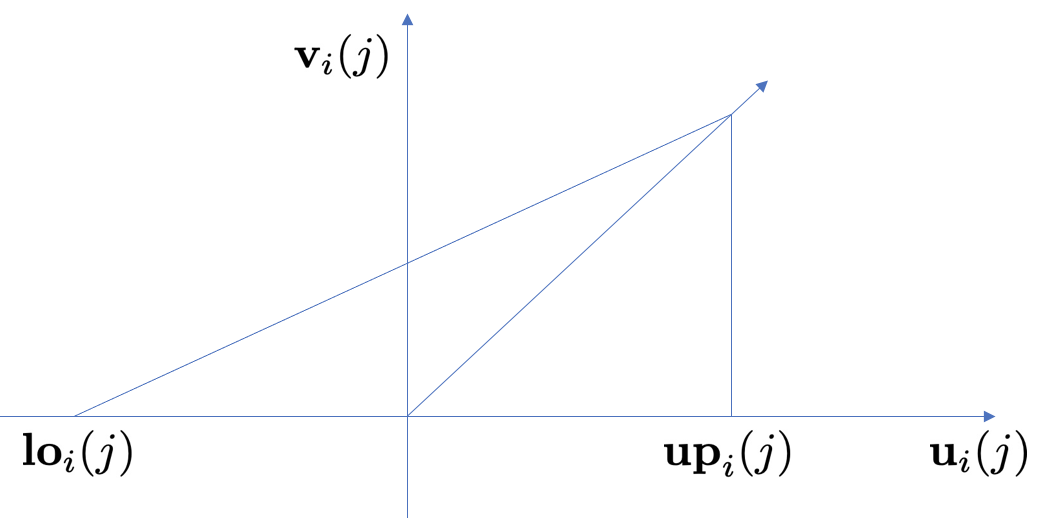
\includegraphics[width=0.7\textwidth]{images/robustnessVerification/ReLUAppro.png}
    \caption{Relaxation of ReLU Activation}
    \label{fig:ReLUApprox}
\end{figure}
Intuitively, when mapping from $\textbf{up}_i(j)$ to $\textbf{v}_i(j)$, instead of using the two lines from ReLU function, i.e., from $(\textbf{lo}_i(j),0)$ to $(0,0)$ and from $(0,0)$ to $(\textbf{up}_i(j),\textbf{up}_i(j))$, we can use the line from $(\textbf{lo}_i(j),0)$ to $(\textbf{up}_i(j),\textbf{up}_i(j))$ to over-approximate the value of $\textbf{v}_i(j)$.  
With this idea, the last three conditions of Equation (\ref{equ:methodtwo}) can be replaced with the below ones for every $j\in [1..s_i]$: 
\begin{equation}\label{equ:MILPapprox}
   \left \{
    \begin{array}{ll}
    \textbf{v}_{i+1}(j)  = 0 & \text{ if } \textbf{up}_{i+1}(j) \leq 0\\
    \textbf{v}_{i+1}(j)  = \textbf{up}_{i+1}(j) & \text{ if } \textbf{lo}_{i+1}(j) \geq 0\\
    \textbf{v}_{i+1}(j)  \geq  0, \textbf{v}_{i+1}(j)  \geq \textbf{up}_{i+1}(j), & \multirow{2}{*}{\text{ otherwise }}\\
    \displaystyle \textbf{v}_{i+1}(j) \leq \frac{\textbf{up}_{i+1}(j)(\textbf{up}_{i+1}(j) - \textbf{lo}_{i+1}(j))}{\textbf{up}_{i+1}(j) - \textbf{lo}_{i+1}(j)} & 
    \end{array}
    \right.
\end{equation}
where the three conditions for the case when $\textbf{up}_{i+1}(j) \geq 0$ and $\textbf{lo}_{i+1}(j) \leq 0$ represent the triangle determined by the three lines such that the value of $\textbf{up}_{i+1}(j)$ will be in the triangle. Therefore, according to the known upper and lower bounds $\textbf{up}_{i+1}(j)$ and $\textbf{lo}_{i+1}(j)$, one of the options in Equation (\ref{equ:MILPapprox})  will be chosen. Note that, all options are linear, without using  any Binary variables. 

Based on the above discussion, if all ReLU activation functions are approximated with Equation (\ref{equ:MILPapprox}), the MILP problem becomes linear programming (LP), which can, in turn, be solved with an LP solver in linear time. We remark that, by approximating the MILP problem (whose computational complexity is NP-complete) with an LP problem (whose computational complexity is in P), solving the optimisation problem becomes tractable, so it is possible to work with a neural network of larger size. 
On the other hand, due to the over-approximation, when we are not able to affirm $d\leq \delta$ as the verification result (as we discussed after Equation (\ref{equ:verification})), we are not able to draw a conclusion on the verification. 

%it is possible that the verification will not return a result when the optimisation problem fails to find a solution.  


\subsection{Computation of Lower and Upper Bounds through Lipschitz Approximation}\label{sec:lowupperbounds}

In this section, we consider how to approximate Lipschitz constant and how to utilise Lipschitz constant for the computation of lower and upper bounds $\textbf{lo}_i$ and $\textbf{up}_i$. Let 
\begin{equation}
    \textbf{G}_i(\textbf{x}) = \displaystyle \frac{\partial \textbf{v}_i}{\partial \textbf{x}} \hspace{1cm}\text{ for } i = 1..K
\end{equation}
be the gradient vector of the hidden activation $\textbf{v}_i$ over the input $\textbf{x}$. 


\subsection*{Approximation of Lipschitz Constant}

We explain how to compute $\textbf{G}_i(\textbf{x})$ by utilising the structural information of the neural network. 
Actually, we will compute both its lower bound $\underline{\textbf{G}}_{i}\in \mathbb{R}^{s_i\times s_1} $ and its upper bound $ \overline{\textbf{G}}_{i}\in \realnumber^{s_i\times s_1}$. 
%
Before proceeding, we define a few notations and operators. Let $[a]_+=\max\{a,0\}$ and $[a]_-=\min\{a,0\}$. For for a matrix $\textbf{F}$, $[\textbf{F}]_+$ and $[\textbf{F}]_-$ are for element-wise max and min. Moreover, we define 
\begin{equation}
    \textbf{W} \otimes [\textbf{lo},\textbf{up}] = [ [\textbf{W}]_+ \times \textbf{lo} + [\textbf{W} ]_- \times \textbf{up}, [\textbf{W}]_+ \times \textbf{up} + [\textbf{W} ]_- \times \textbf{lo}]
\end{equation}
%Moreover, we use $\underline{\textbf{G}}_i\in \realnumber^{s_i\times s_1}$ and $\overline{\textbf{G}}_i\in \real^{s_i\times s_1}$ to denote the lower and upper bound of $\textbf{G}_i$, respectively. 


Actually, we can utilise the chain rule and the sequential structure of the neural network to have the following equation: 
\begin{equation}
    \textbf{G}_i(\textbf{x}) = \frac{\partial \Vec{v}_i}{\partial \Vec{x}} = \frac{\partial \Vec{v}_{i}}{\partial \Vec{u}_{i}}\frac{\partial \Vec{u}_{i}}{\partial \Vec{v}_{i-1}}... \frac{\partial \Vec{v}_{2}}{\partial \Vec{u}_{2}}\frac{\partial \Vec{u}_{2}}{\partial \Vec{v}_{1}}
\end{equation}
which suggests that the gradient $\textbf{G}_i(\textbf{x})$ can be computed repeatedly over the layers. Note that, $\displaystyle\frac{\partial \Vec{u}_{i}}{\partial \Vec{v}_{i-1}}=\textbf{W}_{i-1}$, where $\textbf{W}_{i-1}$ is the weight matrix of layer $i-1$.
Let $\nabla\Vec{\sigma}_i = \displaystyle\frac{\partial \Vec{v}_{i}}{\partial \Vec{u}_{i}}\in \real^{s_{i}\times s_i}$, we have 
\begin{equation}
\textbf{G}_i(\textbf{x}) = \frac{\partial \Vec{v}_i}{\partial \Vec{x}} = \nabla\Vec{\sigma}_{i}\textbf{W}_{i-1}...\textbf{W}_2\nabla\Vec{\sigma}_2\textbf{W}_1
\end{equation}
Let ${\underline{\Lambda}}_i,{\overline{\Lambda}}_i\in \real^{s_i\times s_i}$ be the diagonal matrices denoting the lower and upper bound of $\nabla\Vec{\sigma}_i$, respectively. For ReLU activation function, we have 
\begin{equation}
   \textbf{1} \geq {\overline{\Lambda}}_i\geq {\underline{\Lambda}}_i\geq \textbf{0} 
\end{equation}



To enable a computation of the lower and upper bounds, we use an iterative process as follows. Let $\textbf{F}_{i+1}=\textbf{W}_i\textbf{G}_i$ (i.e., $=\displaystyle\frac{\partial \Vec{u}_{i+1}}{\partial \Vec{x}}$), we have \begin{equation}
    \textbf{G}_i = \nabla\Vec{\sigma}_i\textbf{F}_i = \nabla\Vec{\sigma}_i\textbf{W}_{i-1}\textbf{G}_{i-1}
\end{equation}
The computation proceeds as follows. Initially, we have 
\begin{equation}
    \underline{\textbf{G}}_0 = \overline{\textbf{G}}_0 = \textbf{I}
\end{equation}
where $\textbf{I}$ is the identify matrix. Then, given $\underline{\textbf{G}}_{i-1} $ and $ \overline{\textbf{G}}_{i-1}$, we have 
\begin{equation}
\begin{array}{rll}
    [\underline{\textbf{F}}_{i},\overline{\textbf{F}}_{i}] =  &  \textbf{W}_i \otimes [\underline{\textbf{G}}_{i-1}, \overline{\textbf{G}}_{i-1}] & \\
    \overline{\textbf{G}}_i = & \max \{\underline{\Lambda}_i\overline{\textbf{F}}_i,\overline{\Lambda}_i\overline{\textbf{F}}_i\} = & \overline{\Lambda}_i[\overline{\textbf{F}}_i]_++\underline{\Lambda}_i[\overline{\textbf{F}}_i]_-\\
    \underline{\textbf{G}}_i = & \min \{\underline{\Lambda}_i\underline{\textbf{F}}_i,\overline{\Lambda}_i\underline{\textbf{F}}_i\} = & \underline{\Lambda}_i[\underline{\textbf{F}}_i]_++\overline{\Lambda}_i[\underline{\textbf{F}}_i]_- \\
\end{array}
\end{equation}

Finally, given an input region, which can be either the entire input domain or a $d$-neighbourhood, if we know ${\overline{\Lambda}}_i$ and ${\underline{\Lambda}}_i$, we can compute $[\underline{\textbf{G}}_i, \overline{\textbf{G}}_i]$ with respect to the input region. Therefore, this method can be used to compute either the global Lipschitz constant (when the input region is the entire input domain) or the local Lipschitz constant  (when the input region is a $d$-neighbourhood). 

\subsection*{Computation of Lower and Upper Bounds}

Let $\eta(\textbf{x},L_p,d)$ be a $d$-neighbourhood centred around $\textbf{x}$, we can first use the above method to compute $[\underline{\textbf{G}}_i, \overline{\textbf{G}}_i]$. 
Then,  the upper bound and lower bounds of the $j$-th dimension are as follows: 
\begin{equation}
\begin{array}{cc}
    \textbf{up}_i(j) = & \textbf{v}_i(j) +  \overline{\textbf{G}}_i(j)  \max_{\textbf{x}'\in \eta(\textbf{x},L_p,d)} |\textbf{x}(j) - \textbf{x}'(j)|  \\
    \textbf{lo}_i(j) = & \textbf{v}_i(j) - \underline{ \textbf{G}}_i(j)  \max_{\textbf{x}'\in \eta(\textbf{x},L_p,d)} |\textbf{x}(j) - \textbf{x}'(j)|\\
\end{array}
\end{equation}




\newcommand{\obj}{o}
\newcommand{\off}{w}


%%%%self define math symbol
\def \eg{{\em e.g.,}}
\def \ie{{\em i.e.,}}
\def \etc{{\em etc.}}
\def \mm{{\em mm}}
\def \cm{{\em cm}}
\def \m{{\em m}}
\def \one{{\em i)}}
\def \two{{\em ii)}}
\def \three{{\em iii)}}
\def \four{{\em iv)}}

\def \Safe{\mathrm{S}}
\def \Robust{\mathrm{R}}


\section{Robustness Verification via Reachability Analysis}\label{chap:reachabilityAnalysis}

As discussed in previous chapters, concerns have been raised about the suitability of deep neural networks (DNNs), or systems with DNN components, for deployment in safety-critical applications. 
%To ease this concern and gain users' trust, DNNs need to be certified similarly to %software and hardware  systems such as airplanes and automobiles. 
%
To this end, besides those aforementioned verification techniques, we can also study a generic reachability problem in which, for a given DNN, an input subspace and a function over the network's outputs, computes the upper and lower bounds over the values of the function. The function is generic, with the only requirement that it is Lipschitz continuous. %and has the DNN's output as its input. 
We argue that this problem is fundamental for the certification of DNNs, %can be a core problem towards certifying DNNs 
as it can be instantiated into several key correctness problems, including adversarial example generation \cite{szegedy2014intriguing,DBLP:journals/corr/GoodfellowSS14}, safety verification \cite{HKWW2017,katz2017reluplex,RWSHKK201  8}, and output range analysis \cite{LM2017,dutta2017output}.

%$R_j(X')$ for a given class label $j\in [1..m]$.
% is the set of possible confidence levels $c_j(x)$ over the label $j$. 
% An error bound may be needed for practical reasons. 

To certify a system, a certification approach needs to provide not only a result but also a guarantee over the result, such as the error bounds. 
Existing approaches for analysing DNNs with provable guarantees work by either reducing the problem to a constraint satisfaction problem that can be solved by MILP \cite{LM2017,CNR2017,bunel2017piecewise,xiang2017output}, SAT \cite{NKPSW2017} or SMT \cite{katz2017reluplex,bunel2017piecewise} solvers, or applying search algorithms over discretised vector spaces \cite{HKWW2017,wicker2018feature}. Even though they are able to achieve guarantees, they suffer from two major weaknesses. Firstly, their subjects of study are restricted. 
More specifically, they can only work with layers conducting linear transformations (such as convolutional and fully-connected layers) and simple non-linear transformations (such as ReLU). They cannot work with other important layers, such as the Sigmoid, Max pooling and Softmax layers that are widely used in state-of-the-art networks. Secondly, the scalability of the constraint-based approaches is significantly limited by both the capability of the solvers and the size of the network. However, state-of-the-art networks usually have millions or even billions of hidden neurons. 

This chapter will introduce a novel approach to tackle the generic reachability problem, which does not suffer from the above weaknesses and provides provable guarantees %over its results 
in terms of the upper and lower bounds over the errors. The approach is inspired by recent advances made in the area of global optimisation~\cite{gergel2016adaptive,grishagin2018convergence}. 
For the input subspace defined over a set of input dimensions, an adaptive nested optimisation algorithm is developed. The performance of this algorithm is not dependent on the size of the network, and it can therefore scale to work with large networks. 

This algorithm assumes certain knowledge about the DNN. However, instead of directly translating the activation functions and their parameters (i.e., weights and bias) into linear constraints, % as done in the reduction approaches, 
it needs a Lipschitz constant of the network. For this, we show that several layers that cannot be directly translated into linear constraints are actually Lipschitz continuous, and we can compute a Lipschitz constant by analysing the activation functions and their parameters. This method is implemented as a software tool DeepGO\footnote{It is available on \url{https://github.com/trustAI/DeepGO}.}. 
%and evaluate its performance by comparing with existing constraint-based approaches, namely, SHERLOCK \cite{dutta2017output} and Reluplex \cite{katz2017reluplex}. We also demonstrate % on several problems that can be handled by them. Our experiments include those networks that cannot be handled by existing algorithms. 
% our tool on DNNs that are beyond the capability of existing tools.

%Practically, the layer-to-layer mapping functions can be various types of activation functions such as ReLU, Leaky ReLU, sigmoid function, Hyperbolic tangent function etc., or different pooling operations such as max pooling and contrast-normalization pooling, and softmax layer (usually in the last layer). Noted that existing methods of reachability analysis for DNNs are all based on MLP [?], SAT [?] or SMT [?] techniques, which enable them has the following three major limitations: \one~they are only workable on the ReLU activation functions due to the linearizion formulation; \two~they cannot analyses softmax layer which enables their reachability analysis not complete; and \three~those methods are based on a layer-by-layer analysis which makes them only workable for a small-scale neural network(such as 3-layer NN with only hundreds of neurons. 

%To deal with the above limitation, in this paper, we tackle the problem from a "black-box" point of view, which is neither depends on the layer-by-layer analysis nor built upon any MLP solvers. The only assumption we rely on is that the targeted deep neural network satisfies the Lipschitz continuity assumption.
		%\vspace{1mm}

%\vspace{-3pt}

\subsection{Lipschitz Continuity of Deep Learning}\label{sec:lipschitz}

This section shows that feed-forward DNNs are Lipschitz continuous.
Let $f: \mathbb{R}^n \rightarrow \mathbb{R}^m$ be a $N$-layer 
%feed-forward neural 
network such that, for a given input $\mathbf{x}\in \mathbb{R}^n$, $f(\mathbf{x}) = \{c_1,c_2,...,c_m\}\in \mathbb{R}^m$ represents the confidence values for $m$ classification labels. Specifically, we have 
$f(\mathbf{x}) = f_N(f_{N-1}(...f_1(\mathbf{x};\mathbf{W}_1,\mathbf{b}_1);\mathbf{W}_2,\mathbf{b}_2);...);\mathbf{W}_N,\mathbf{b}_N)
$ where $\mathbf{W}_i$ and $\mathbf{b}_i$ for $i = 1,2,...,N$ are learnable parameters and $f_i(\mathbf{z}_{i-1};\mathbf{W}_{i-1},\mathbf{b}_{i-1})$ is the function mapping from the output of layer $i-1$ to the output of layer $i$ such that $\mathbf{z}_{i-1}$ is the output of layer $i-1$. Without loss of generality, we normalise the input $\mathbf{x}\in [0,1]^n$. The output $f(\mathbf{x})$ is usually normalised to be in $[0,1]^m$ with a Softmax layer. 
	


\begin{definition}[Lipschitz Continuity]
	Given two metric spaces $(\mathbf{X}, d_\mathbf{X})$ and $(\mathbf{Y}, d_\mathbf{Y})$, where $d_\mathbf{X}$ and $d_\mathbf{Y}$ are the metrics on the sets $\mathbf{X}$ and $\mathbf{Y}$ respectively, a function $f: \mathbf{X}\rightarrow \mathbf{Y}$ is called {\em Lipschitz continuous} if there exists a real constant $K\geq0$ such that, for all $\mathbf{x}_1, \mathbf{x}_2 \in \mathbf{X}$:
	\begin{equation}
	 d_\mathbf{Y}(f(\mathbf{x}_1), f(\mathbf{x}_2)) \le K d_\mathbf{X}(\mathbf{x}_1, \mathbf{x}_2).
	\end{equation}
	$K$ is called the {\em Lipschitz constant} for the function $f$. The smallest $K$ is called {\em the Best Lipschitz constant}, denoted as $K_{best}$.
\end{definition}

The work in \cite{szegedy2014intriguing} shows that deep neural networks with half-rectified layers (\ie~convolutional or fully connected layers with ReLU activation functions), max pooling and contrast-normalization layers are Lipschitz continuous. They prove that the upper bound of the Lipschitz constant can be estimated via the operator norm of learned parameters $\mathbf{W}$. Furthermore, other researchers theoretically demonstrate that the Softmax layer, Sigmoid and Hyperbolic tangent activation functions also satisfy the Lipschitz continuity, the details of the proof can be found in the work of \cite{RHK2018}.

% First we need the following lemma~\cite{sohrab2003basic}.

% \begin{mylemma}\label{theo-1}
% Let $f: \mathbb{R}^n \rightarrow \mathbb{R}^m$,	if $||\partial{f(\mathbf{x})}/\partial{\mathbf{x}}|| \leq K$ for all $\mathbf{x} \in [\mathbf{a}, \mathbf{b}]^n$, then $f$ is Lipschitz continuous on $[\mathbf{a}, \mathbf{b}]^n$ and $K$ is its Lipschitz constant, where $||*||$ represents a norm operator.
% \end{mylemma}

% Based on this lemma, we have the following theorem.

% \begin{theorem}
% Convolutional or fully connected layers with the sigmoid activation function $s(W\mathbf{x}+b)$, Hyperbolic tangent activation function $t(W\mathbf{x}+b)$, and softmax function $p(\mathbf{x})_j$ are Lipschitz continuous and their Lipschitz constants are $\dfrac{1}{2}\norm{W}$, $\norm{W}$, and $\sup_{i,j}(\norm{\mathbf{x}_i} + \norm{\mathbf{x}_i\mathbf{x}_j})$, respectively.
% \end{theorem}

% \begin{myproof}
% First of all, we show that the norm operators of their Jacobian matrices are bounded.

% (1)~Layer with sigmoid activation $s(q) = 1/(1+e^{-q})$ with $ q = W\mathbf{x}+b$:
% \begin{equation}
% \begin{split}
% \norm{\dfrac{\partial{s(\mathbf{x})}}{\partial{\mathbf{x}}}} = \norm{\dfrac{\partial{s(q)}}{\partial{q}} \dfrac{\partial{q}}{\partial{\mathbf{x}}}}
% \leq \norm{\dfrac{\partial{s(q)}}{\partial{q}}} \norm{\dfrac{\partial{q}}{\partial{\mathbf{x}}}}\\
% \leq \norm{s(q)\circ(\mathbf{1}-s(q))}\norm{W}\leq \dfrac{1}{4}\norm{W}
% \end{split}
% \end{equation}

% (2)~Layer with Hyperbolic tangent activation function $t(q) = 2/(1+e^{-2q})-1$ with $ q = W\mathbf{x}+b$:
% \begin{equation}
% \begin{split}
% \norm{\dfrac{\partial{t(\mathbf{x})}}{\partial{\mathbf{x}}}} = \norm{\dfrac{\partial{t(q)}}{\partial{q}} \dfrac{\partial{q}}{\partial{\mathbf{x}}}}
% \leq \norm{\dfrac{\partial{t(q)}}{\partial{q}}} \norm{\dfrac{\partial{q}}{\partial{\mathbf{x}}}}\\
% \leq \norm{\mathbf{1}-t(q)\circ t(q))}\norm{W}\leq \norm{W}
% \end{split}
% \end{equation}

% (3)~Layer with softmax function $p(\mathbf{x})_j = e^{\mathbf{x}_j}/(\sum_{k = 1}^{n}{e^{\mathbf{x}_k}})$ for $j = 1,...,m$ and $n = m$ (dimensions of input and output of softmax are the same):
% \begin{equation}
% \begin{split}
% \norm{\dfrac{\partial{p(\mathbf{x})_j}}{\partial{\mathbf{x}_i}}} = 
% \left\{
% \begin{array}{ll}
% \mathbf{x}_i(1-\mathbf{x}_j), ~~i = j\\
% -\mathbf{x}_i\mathbf{x}_j,~~i\ne j
% \end{array}
% \right. \leq \sup_{i,j} (\norm{\mathbf{x}_i} + \norm{\mathbf{x}_ix_j})
% \end{split}
% \end{equation}
% Since the softmax layer is the last layer of a deep neural network, we can estimate its supremum based on Lipschitz constants of previous layers and box constraints of DNN's input.

% The final conclusion follows by Lemma 1 and the fact that all the layer functions are bounded on their Jacobian matrix. 
% \end{myproof}


\subsection{Reachability Analysis of Deep Learning}

In this section, we present the formulate the problem of confidence reachability of a neural network. 
Let $\obj: [0,1]^m \rightarrow \mathbb{R}$ be a Lipschitz continuous function statistically evaluating the outputs of the network. Our problem is to find its upper and lower bounds given the set $\mathbf{X}'$ of inputs to the network. Because both the network $f$ and the %statistical evaluation 
function $\obj$ are Lipschitz continuous, all values between the upper and lower bounds have a corresponding input, i.e., are reachable. 

\begin{definition}[Reachability of Neural Network]
Let $\mathbf{X}'\subseteq [0,1]^n$ be an input subspace and $f: \mathbb{R}^n \rightarrow \mathbb{R}^m$ a network.
% such that $f(x) = \{c_1,...,c_j,...,c_m\}\in [0,1]^m$ and $c_j$ is the $j$-th confidence output representing the probability of input $x$ belonging to $j$-th classification label. We also use $c_j(x)$ to represent the $j$-th output of DNN given input $x$. Then 
The reachability of $f$ over the function $\obj$ under an error tolerance $\epsilon \geq 0$ is a set $R(\obj,\mathbf{X}',\epsilon) = [l,u]$ such that 
\begin{equation}
\begin{split}
\inf_{\mathbf{x}' \in \mathbf{X}'} \obj(f(\mathbf{x}')) -\epsilon \leq l \leq \inf_{\mathbf{x}' \in \mathbf{X}'} \obj(f(\mathbf{x}')) +\epsilon \\
\sup_{\mathbf{x}' \in \mathbf{X}'} \obj(f(\mathbf{x}')) - \epsilon \leq u \leq \sup_{\mathbf{x}' \in \mathbf{X}'} \obj(f(\mathbf{x}')) + \epsilon.
\end{split}
\end{equation}
We write $u(\obj,\mathbf{X}',\epsilon)=u$ and $l(\obj,\mathbf{X}',\epsilon)=l$ for the upper and lower bound, respectively. 
%Confidence Upper Bound (CUB) and Confidence Lower Bound (CLB), respectively. 
Then the reachability diameter is 
	\begin{equation}
           D(\obj,\mathbf{X}',\epsilon) =u(\obj,\mathbf{X}',\epsilon)-l(\obj,\mathbf{x}',\epsilon).
	\end{equation}
Assuming these notations, we may write $D(\obj,\mathbf{X}',\epsilon;f)$ if we need to explicitly refer to the network $f$. 
\end{definition}

In the following, we instantiate $\obj$ with a few concrete functions, and show that several key verification problems for DNNs can be reduced to our reachability problem. 

\begin{definition}[Output Range Analysis]
Given a class label $j\in [1,..,m]$, we let $\obj = \Pi_j$ such that $\Pi_j((c_1,...,c_m))=c_j$. 
\end{definition}

We write $c_j(\mathbf{x}) = \Pi_j(f(\mathbf{x}))$ for the network's confidence in classifying $\mathbf{x}$ as label $j$. 
Intuitively, output range \cite{dutta2017output} quantifies how a certain output of a deep neural network (\ie~classification probability of a certain label $j$) varies in response to a set of DNN inputs with an error tolerance $\epsilon$. Output range analysis can be easily generalised to logit \footnote{Logit output is the output of the layer before the softmax layer. The study of logit outputs is conducted in, e.g., \cite{dutta2017output}.} range analysis.

We show that the safety verification problem \cite{HKWW2017} can be reduced to solving the reachability problem. 

\begin{definition}[Local Safety]
A network $f$ is safe with respect to an input $\mathbf{x}$ and an input subspace $\mathbf{X}'\subseteq [0,1]^n$ with $\mathbf{x} \in \mathbf{X}'$, written as $\Safe(f,\mathbf{x},\mathbf{X}')$, if 
\begin{equation}
\forall \mathbf{x}' \in \mathbf{X}': \arg\max_{j} c_j(\mathbf{x}') = \arg\max_{j} c_j(\mathbf{x})
\end{equation} 
%where $c_j(x) = f(x)_j$ returns $N$'s confidence in classifying $x$ as label $j$. 
\end{definition}

We have the following reduction theorem. 

%For the reduction, we define two functions $o_1=\Pi_j$ such that $j=\arg\max_{j}c_j(x)$, and $o_2 = +_{-j}$ such that $+_{-j}(c_1,...,c_m) = \sum_{i=1, i\neq j}^{m} c_i$. Therefore, we have 

\begin{theorem}\label{thm:safety}
A network $f$ is safe with respect to $\mathbf{x}$ and $\mathbf{X}'$ s.t. $\mathbf{x} \in \mathbf{X}'$ if and only if
$u(\oplus,\mathbf{X}',\epsilon) \leq 0$,
%$l(\Pi_j,X',\epsilon) \geq u(\oplus_{-j},X',\epsilon)$
where $\oplus(c_1,...,c_m) = \max_{i\in \{1..m\}}(\Pi_{i} (c_1,...,c_m) - \Pi_{j} (c_1,...,c_m))$ and $j=\arg\max_{j}c_j(\mathbf{x})$. The error bound of the safety decision problem by this reduction is $2\epsilon$. 
\end{theorem}

It is not hard to see that the adversarial example generation \cite{szegedy2014intriguing}, which is to find an input $\mathbf{x}' \in \mathbf{X}'$ such that $\arg\max_{j} c_j(\mathbf{x}') \neq \arg\max_{j} c_j(\mathbf{x})$, is the dual problem of the safety problem. 

% The following two problems define the robustness comparisons between the networks and/or the inputs. 

% \begin{definition}[Model Robustness Comparison]
% Given two homogeneous\footnote{Here, two networks are homogeneous if they are applied on the same classification task but may have different network architectures (e.g., layer numbers, layer types, etc) and/or parameters.}
% %E.g., two different neural networks but both are for the MNIST image classification task.} 
% networks $f$ and $g$, we say that model $f$ is strictly more robust than model $g$ with respect to a function $\obj$, an input subspace $\mathbf{X}'$ and an error bound $\epsilon$, written as $\Robust_{o,\mathbf{X}',\epsilon}(f,g)$, if $D(\obj,\mathbf{X}',\epsilon;f) < D(\obj,\mathbf{X}',\epsilon;g)$.

% %$j$-th output and an input subspace $\bar{x}$ if $D_j(\bar{x};f(x)) < D_j(\bar{x};g(x))$.
% \end{definition}

% \begin{definition}[Subspace Robustness Comparison]
% 	Given two input sub-spaces $\mathbf{X}'$ and $\mathbf{X}''$ and a network $f$, we say that $f$ is more robust on subspace $\mathbf{X}'$ than on subspace $\mathbf{X}''$ with respect to a statistical function $\obj$ and an error bound $\epsilon$, written as $\Robust_{f,o,\epsilon}(\mathbf{X}',\mathbf{X}'')$, if $D(\obj,\mathbf{X}',\epsilon) < D(\obj,\mathbf{X}'',\epsilon)$.
% %$D_j(\bar{x}) < D_j(\hat{x})$.
% \end{definition}

Thus, by instantiating the function $\obj$, we can quantify a network's output/logit range and verify whether a network is robust or safe.
		%\vspace{-1mm}

%\vspace{-3pt}
\subsection{Confidence Reachability with Guarantees}
%\vspace{-1pt}

Section~\ref{sec:lipschitz} shows that a deep feedforward neural network is Lipschitz continuous regardless of its layer depth, activation functions and the number of neurons. Now, to solve the reachability problem, we need to find the \emph{global} minimum and maximum values given an input subspace, assuming that we have a Lipschitz constant $K$ for the function $o\!\cdot\!f$. In the following, we let $\off = o\!\cdot\!f$ be the concatenated function. Without loss of generality, we assume the input space $\mathbf{X}'$ is a box-constraint (i.e., measured by $L_\infty$-norm distance), which is clearly feasible since images are usually normalised into $[0,1]^n$ before being fed into a neural network.

% Thus we need to solve the following problem. Here we start to use $x$ instead of $\bar{x}$ (we can treat the fixed dimensions in input space as a learned parameters in neural network) and drop index $j$ (since we can perform the some analysis to each output separately). 
The computation of the minimum value is reduced to solving the following optimisation problem with guaranteed convergence to the global minimum (the maximisation problem can be similarly solved by minimising the negative objective function):
\begin{equation}\label{equ-8}
\begin{split}
\min\limits_{\mathbf{x}}~~\off(\mathbf{x}),~~~s.t.~~\mathbf{x} \in [a,b]^n
\end{split}
\end{equation}
However, the above optimisation is very challenging since $\off(\mathbf{x})$ is a highly non-convex function which cannot be guaranteed to reach the global minimum by regular optimisation schemes based on gradient descent. Inspired by an idea from optimisation, e.g., \cite{piyavskii1972algorithm,TZ1989}, we design another continuous function $h(\mathbf{x},\mathbf{y})$, which serves as a lower bound of the original function $\off(\mathbf{x})$. Specifically, we need 
%This idea is also widely adopted in optimization community.
\begin{equation}\label{equ-9}
\begin{split}
\forall \mathbf{x}, \mathbf{y} \in [a,b]^n,~ h(\mathbf{x},\mathbf{y}) \leq \off(\mathbf{x})~~\text{and}~~h(\mathbf{x},\mathbf{x}) = \off(\mathbf{x})
\end{split}
\end{equation}
%
Furthermore, for $i\geq 0$, we let $\mathcal{Y}_i = \{\mathbf{y}_0,\mathbf{y}_1,...,\mathbf{y}_i\} $ be a finite set containing $i+1$ points from the input space $ [a, b]^n$, and let $\mathcal{Y}_i \subseteq \mathcal{Y}_k$ when $k>i$, then we can define a function
$H(\mathbf{x};\mathcal{Y}_i) = \max_{\mathbf{y}\in \mathcal{Y}_i } h(\mathbf{x},\mathbf{y})$
 which satisfies the following relation:
\begin{equation}
H(\mathbf{x}; \mathcal{Y}_i) < H(\mathbf{x}; \mathcal{Y}_k)\leq %\inf_{x\in [a,b]^n}
\off(\mathbf{x}), \forall i < k
\end{equation}

We use $l_i = \inf_{\mathbf{x}\in [a,b]^n} H(\mathbf{x};\mathcal{Y}_i)$ to denote the minimum value of $H(\mathbf{x};\mathcal{Y}_i)$ for $\mathbf{x}\in [a,b]^n$. Then we have 
%can get the following relation:
\begin{equation}
l_0< l_1< ... < l_{i-1}< l_i \leq \inf_{\mathbf{x}\in [a,b]^n} \off(\mathbf{x})
\end{equation}
Similarly, we need a sequence of upper bounds $u_i$ to have 
\begin{equation}\label{eqn-14}
\begin{split}
l_0< ... < l_i \leq \inf_{\mathbf{x}\in [a,b]^n} \off(\mathbf{x})\leq u_i< ...< u_0
\end{split}
\end{equation}
By Expression (\ref{eqn-14}), we can have the following:
\begin{equation}\label{eqn-15}
\begin{split}
\lim\limits_{i\to \infty}l_i = \min_{\mathbf{x}\in [a,b]^n} \off(\mathbf{x}) \text{   and   }
\lim\limits_{i\to \infty}(u_i - l_i) = 0
\end{split}
\end{equation}

Therefore, we can asymptotically approach the global minimum. Practically, we execute a finite number of iterations by using an error tolerance $\epsilon$ to control the termination. 
%
%\begin{myremarks}
%	Whenever terminated, it returns a lower bound and a upper bound of the global minimum, and we can evaluate the quality of global minimum obtained so far.
%\end{myremarks}
%
In the next section, we present the approach, which constructs a sequence of lower and upper bounds, and show that it can converge with an arbitrarily-small error bound. 
%To handle the high-dimensionality of DNNs, our approach is inspired by the idea of adaptive nested optimisation in \cite{gergel2016adaptive}, with significant differences in the detailed algorithm and convergence proof. 

%We first discuss the one-dimension case and then the multiple-dimension case.
\begin{figure}[t]
	\centering
	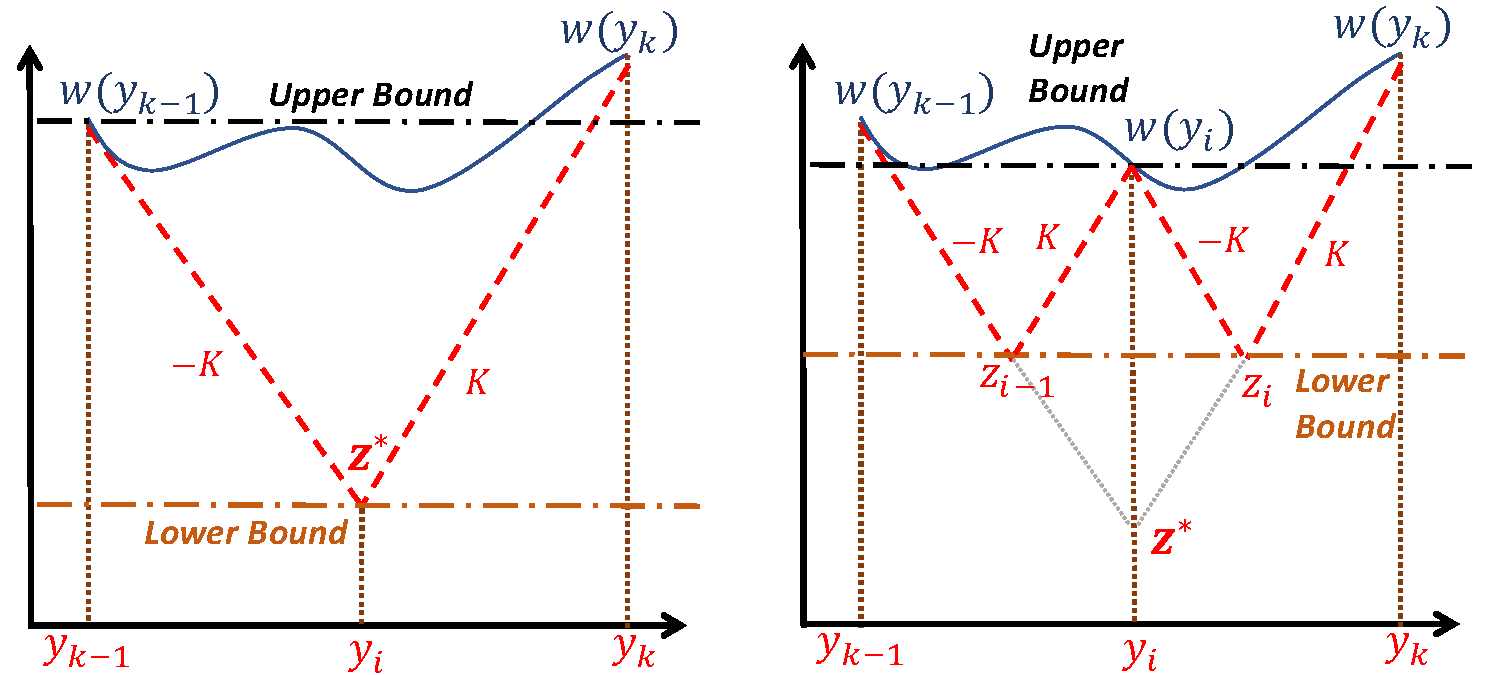
\includegraphics[width=1\linewidth]{images/robustnessVerification/f1.pdf}
	\caption{A lower-bound function designed via Lipschitz constant}
	\label{fig-1}
\end{figure}


\subsubsection{One-dimensional Case}\label{sec:onedimensional}


We first introduce an algorithm which works over one dimension of the input, and therefore is able to handle the case of $x \in [a,b]$ in Eqn.~(\ref{equ-8}).
%, based on Section 2 and Theorem~1, we can estimate the Lipschitz constants of a neural network numerically either or analytically. 
The multi-dimensional optimisation algorithm will be discussed in the next section by repeatedly utilising the one-dimensional algorithm. 
We define the following lower-bound function.
\begin{equation}\label{eqn-10}
\begin{split}
h({x},y) = \off(y) - K|{x}-y| \\
H({x};\mathcal{Y}_i) = \max\limits_{y\in \mathcal{Y}_i }~~\off(y) - K|{x}-y|
\end{split}
\end{equation}
where $K > K_{best}$ is a Lipschitz constant of $\off$ and $H({x};\mathcal{Y}_i)$ intuitively represents the lower-bound saw-tooth function shown as Fig.~\ref{fig-1}.
%$L \geq K_{best}$ and we can estimate by $L = |d(c(x))/dx| + \eta$ $(\eta \geq 0)$ based on Theorem~1. 
The set of points $\mathcal{Y}_i$ is constructed recursively. Assuming that, after $(i-1)$-th iteration, we have $\mathcal{Y}_{i-1} = \{y_0,y_1,..,y_{i-1}\}$, whose elements are in ascending order, and sets 
$$
\off(\mathcal{Y}_{i-1} )=\{\off(y_0), \off(y_1),..,\off(y_{i-1})\}
$$
$$\mathcal{L}_{i-1} = \{l_0,l_1,...,l_{i-1}\}$$
$$\mathcal{U}_{i-1} = \{u_0,u_1,...,u_{i-1}\}$$
$$\mathcal{Z}_{i-1} = \{z_1,...,z_{i-1}\}$$
%where $z_{k} = \dfrac{\off(y_{k})+ \off(y_{k-1})}{2} - \dfrac{K(y_{k} - y_{k-1})}{2}, \forall k = 1,2,..,i-1$. 
%
The elements in sets $\off(\mathcal{Y}_{i-1} )$, $\mathcal{L}_{i-1}$ and $\mathcal{U}_{i-1}$ have been defined earlier. The set $\mathcal{Z}_{i-1}$ records the smallest values $z_k$ computed in an interval $[y_{k-1},y_k]$.

In $i$-th iteration, we do the following sequentially:
\begin{itemize}

%\item Numerically estimate Lipschitz constant as $K = \eta \max_{j = 1,...,i-1} \{(\off(y_j) - \off(y_{j-1}))/(y_j - y_{j-1})\}$ where $\eta > 1$.

	\item Compute $y_i = \arg\inf_{{x}\in [a,b]} H({x};\mathcal{Y}_{i-1})$ as follows. Let $z^* = \min{\mathcal{Z}_{i-1} }$ and $k$ be the index of the interval $[y_{k-1},y_k]$ where $z^*$ is computed. Then we let 
\begin{equation}\label{equ:newpoint}
y_i = \dfrac{y_{k-1}+y_k}{2} - \dfrac{\off(y_{k}) - \off(y_{k-1})}{2K}
\end{equation}

 and have that $y_i \in (y_{k-1},y_k)$. 
	
	\item Let $\mathcal{Y}_i = \mathcal{Y}_{i-1}\cup\{y_i\}$, then reorder $\mathcal{Y}_i$ in ascending order, and update $\off(\mathcal{Y}_{i} )=\off(\mathcal{Y}_{i-1})\cup \{\off(y_i)\}$.
	
	\item Calculate 
	\begin{equation}\label{eqn-16}
	z_{i-1} = \dfrac{\off(y_{i})+ \off(y_{k-1})}{2} - \dfrac{K(y_{i} - y_{k-1})}{2}\end{equation}
	
	\begin{equation}\label{eqn-17}
	z_{i} = \dfrac{\off(y_{k})+ \off(y_{i})}{2} - \dfrac{K(y_{k} - y_{i})}{2}\end{equation} and update $\mathcal{Z}_{i} = (\mathcal{Z}_{i-1}\setminus \{z^*\}) \cup\{z_{i-1},z_{i}\} $.
	
	\item Calculate the new lower bound $l_i = \inf_{{x}\in [a,b]} H({x};\mathcal{Y}_i)$ by letting $l_i =\min\mathcal{Z}_{i}$,
%\min \{l_{i-1}, z_{i-1},z_{i}\}$, 
and updating $\mathcal{L}_{i} = \mathcal{L}_{i-1} \cup \{l_i \}$.
	
	\item Calculate the new upper bound $u_i = \min_{y\in \mathcal{Y}_i }\off(y)$ by letting $u_i = \min \{u_{i-1}, \off(y_i)\}$.
\end{itemize}

We terminate the iteration whenever $|u_i-l_i|\leq\epsilon$,
% where $\epsilon$ is the error tolerance, 
and let the global minimum value be $y^* = \min_{{x}\in [a,b]} H({x};\mathcal{Y}_{i})$ and the minimum objective function be $\off^* = \off(y^*)$. 

Intuitively, as shown in Fig.~\ref{fig-1}, the key idea in this algorithm is to design a piecewise-linear lower bound function, which is guaranteed to be underneath the original function because of Lipschitz continuity. This lower bound function is refined iteration by iteration until the stopping criteria are satisfied. In each iteration, this algorithm is able to generate lower bounds by calculating the lowest point of the lower bound function; the upper bound is the lowest evaluation value of the original function so far. 

% \subsection{Convergence Analysis}
% In the following, we show the convergence of this algorithm to the global minimum by proving the following conditions. 
% \begin{itemize}
%     \item Convergence Condition 1: $\lim\limits_{i\to \infty}l_i = \min\limits_{\mathbf{x}\in [a,b]} \off(\mathbf{x})$
%     \item Convergence Condition 2: $\lim_{i\to \infty}(u_i - l_i) = 0$
% \end{itemize}

% \begin{myproof}[Monotonicity of Lower/Upper Bound Sequences]
% First, we prove that the lower bound sequence $\mathcal{L}_i$ is strictly monotonic. 
% 	Because 
% 	\begin{equation}l_i = \min \mathcal{Z}_i= \min \{(\mathcal{Z}_{i-1}\setminus \{z^*\}) \cup\{z_{i-1},z_{i}\} \} \end{equation} and $l_{i-1} = \min \mathcal{Z}_i$. To show that $l_i > l_{i-1}$, we need to prove $z_{i-1} > z^*$ and $z_{i} > z^*$. By the algorithm, $z^*$ is computed from interval $[y_{k-1}, y_k]$, so we have %
% 	\begin{equation}\label{eqn-19}
% 	z^* = \dfrac{\off(y_{k})+ \off(y_{k-1})}{2} - \dfrac{K(y_{k} - y_{k-1})}{2}\end{equation}
% 	We then have 
% 	\begin{equation}\label{equ:lowerbound}
% 	z_{i-1} - z^* = \dfrac{\off(y_i)-\off(y_k) - K(y_i - y_k)}{2}
% 	\end{equation} 
% 	Since $y_i < y_{k}$ and $K>K_{best}$, by Lipschitz continuity we have $z_{i-1} > z^* $. 
% 	Similarly, we can prove $z_{i} > z^* $. Thus $l_i > l_{i-1}$ is guaranteed. 
	
% 	Second, the monotonicity of upper bounds $u_i$ can be seen from the algorithm, since $u_i $ is updated to $ \min \{u_i, \off(y_i)\}$ in every iteration. 
% \label{proof2}
% \end{myproof}

% \begin{myproof}[Convergence Condition 1]
% 	~\\
% 	Since $\mathcal{Y}_{i-1}\subseteq \mathcal{Y}_{i}$, we have $H(\mathbf{x}; \mathcal{Y}_{i-1}) \leq H(\mathbf{x}; \mathcal{Y}_{i})$. Based on Proof~\ref{proof2}, we also have $l_{i-1}< l_i$. Then since  %And because 
% 	\begin{equation}l_i = \inf_{\mathbf{x}\in [a,b]} H(\mathbf{x}; \mathcal{Y}_{i}) \leq \min_{\mathbf{x}\in [a,b]}\off(\mathbf{x})\end{equation} 
% 	the lower bound sequence $\{l_0,l_1,...,l_i\}$ is strictly monotonically increasing and bounded from above by $\min_{\mathbf{x}\in [a,b]}\off(\mathbf{x})$. Thus $\lim_{i\to \infty}l_i = \min_{\mathbf{x}\in [a,b]} \off(\mathbf{x})$ holds.
% \end{myproof}



% \begin{myproof}[Convergence Condition 2]
% 	~\\
% 	Since $\lim_{i\to \infty}l_i = \min_{\mathbf{x}\in [a,b]} \off(\mathbf{x})$, we show $\lim_{i\to \infty}(u_i - l_i) = 0$ by showing that $\lim_{i\to \infty}u_i = \min_{\mathbf{x}\in [a,b]} \off(\mathbf{x})$. 
% Since $\mathcal{Y}_{i} = \mathcal{Y}_{i-1} \cup\{y_i\}$ and $y_i \in X =[a, b]$, we have $\lim_{i\to \infty} \mathcal{Y}_{i} = X$. Then we have $\lim_{i\to \infty}u_i = \lim_{i\to \infty} \inf_{y\in \mathcal{Y}_i } \off(y) = \inf {\off(X)}$. Since $X = [a,b]$ is a closed interval, we can prove $\lim_{i\to \infty}u_i = \inf {\off(X)} = \min_{\mathbf{x}\in [a,b]} \off(\mathbf{x})$. 
% \end{myproof}

%\begin{equation}K = \eta \max_{j = 1,...,i-1} \abs{\dfrac{\off(y_j) - \off(y_{j-1})}{y_j - y_{j-1}}}\end{equation} where $\eta > 1$. We emphasise that, because 


\subsubsection{Dynamically Improving the Lipschitz Constant}

A Lipschitz constant closer to $K_{best}$ can greatly improve the speed of convergence of the algorithm. We design a practical approach to dynamically update the current Lipschitz constant according to the information obtained from the previous iteration: 
\begin{equation}
K = \eta \max_{j = 1,...,i-1} \bigg |{\dfrac{\off(y_j) - \off(y_{j-1})}{y_j - y_{j-1}}}\bigg |
\end{equation} 
where $\eta > 1$. We emphasise that, with the optimisation proceeds, the more evaluations on the objective function we have, a more accurate estimation of the Lipschitz constant we can obtain, i.e., 
%during the iteration, we can numerically approximate the Lipschitz constant $K$, as we can show that 
$$ \lim_{i \to \infty} \max_{j = 1,...,i-1} \eta\bigg |{\dfrac{\off(y_j) - \off(y_{j-1})}{y_j - y_{j-1}}}\bigg | = \eta \sup_{y\in [a,b]} \bigg |{\dfrac{d\off}{dy}}\bigg | > K_{best}
$$
The above analysis indicates that this dynamic estimation strategy can eventually approximate the true Lipschitz constant when iteration number $i$ approximates to infinity.

\subsubsection{Multi-dimensional Case}

%We 
%use the nested optimization approach, which is widely applied in optimization community~\cite{gergel2016adaptive}. Its core idea is to
The basic idea is to decompose a multi-dimensional optimisation problem into a sequence of nested one-dimensional sub-problems. Then the minima of those one-dimensional minimisation sub-problems are back-propagated into the original dimension and the final global minimum is obtained. 
\begin{equation}\label{equ-16}
\min\limits_{\mathbf{x} \in [a_i,b_i]^n}~~\off(\mathbf{x}) =
\min\limits_{{x}_1\in [a_1,b_1]}... \min\limits_{{x}_n\in [a_n,b_n]} \off({x}_1,...,{x}_n)
\end{equation}

We first introduce the $k$-th level sub-problem.

\begin{definition}\label{def:kthlevel}
%[$k$-th Level Subproblem]
	The $k$-th level optimisation sub-problem, written as $\phi_k({x}_1,...,{x}_k)$, is defined as follows: for $1\leq k \leq n-1$,
	%
	$$\phi_k({x}_1,...,{x}_k) = \min_{{x}_{k+1}\in [a_{k+1},b_{k+1}]} \phi_{k+1}({x}_1,...,{x}_k, {x}_{k+1}) $$
	%
	and for $k=n$, $$\phi_n({x}_1,...,{x}_n) = \off({x}_1,{x}_2,...,{x}_n).$$
\end{definition}
%
Combining Expression (\ref{equ-16}) and Definition~\ref{def:kthlevel}, we have that $$\min_{{\mathbf{x}} \in [a_i,b_i]^n}~~\off({\mathbf{x}}) = \min_{{x}_1\in [a_1,b_1]} \phi_1({x}_1)$$ which is actually a one-dimensional optimisation problem and therefore can be solved by the method in Section~\ref{sec:onedimensional}. 

However, when evaluating the objective function $\phi_1({x}_1)$ at ${x}_1=a_1$, we need to project $a_1$ into the next one-dimensional sub-problem $$\min_{{x}_2\in [a_2,b_2]}\phi_2(a_1,{x}_2)$$ We recursively perform the projection until we reach the $n$-th level one-dimensional sub-problem, $$\min_{{x}_n\in [a_n,b_n]}\phi_n(a_1, a_2,..., a_{n-1},{x}_n)$$ 
Once solved,
% all one-dimension subproblems, 
we back-propagate objective function values to the first-level $\phi_1(a_1)$ and continue searching from this level until the error bound is reached.

The convergence analysis for both one-dimensional and multi-dimensional cases can be referred from \cite{RHK2018}. Here we point out that, the proof in \cite{RHK2018} indicates that the overall error bound of the nested scheme only increases linearly w.r.t. the bounds in the one-dimensional case. 

% And an adaptive approach can be applied to optimise its performance without compromising convergence. The
% key observation is to relax the strict subordination inherent in the nested scheme and 
% simultaneously consider all the univariate subproblems arising in the course of
% multidimensional
% optimization.
% %
% For all the generated subproblems that are active, a numerical measure is applied.
% Then an iteration of the multidimensional optimization consists in choosing the subproblem
% with maximal measurement and carrying out a new trial within this subproblem.
% The measure is defined to be the maximal interval characteristics generated by the one-dimensional optimisation algorithm. 


% \subsection{Empirical Study}

% Two methods are chosen as baseline methods in this paper:
% \begin{itemize}
%     \item Reluplex~\cite{katz2017reluplex}: an SMT-based method for solving queries on DNNs with ReLU activations; we apply a bisection scheme to compute an interval until an error is reached
%     \item SHERLOCK~\cite{dutta2017output}: a MILP-based method dedicated to output range analysis on DNNs with ReLU activations.
% \end{itemize}

% Our software is implemented in Matlab 2018a, running on a notebook computer with i7-7700HQ CPU and 16GB RAM. Since Reluplex and SHERLOCK (not open-sourced) are designed on different software platforms, we take their experimental results from~\cite{dutta2017output}, whose experimental environment is a Linux workstation with 63GB RAM and 23-Cores CPU (more powerful than ours) and $\epsilon=0.01$.
% %
% Following the experimental setup in~\cite{dutta2017output}, we use their data (2-input and 1-output functions) to train six neural networks with various numbers and types of layers and neurons. The input subspace is $X' = [0,10]^2$. 

% The comparison results are given in Fig.~\ref{fig-2}. 
% They show that, while the performance of both Reluplex and SHERLOCK is considerably affected by the increase in the number of neurons and layers, our method is not. For the six benchmark neural networks, our average computation time is around $5s$, 36 fold improvement over SHERLOCK and nearly 100 fold improvement over Reluplex (excluding timeouts). We note that our method is running on a notebook PC, which is significantly less powerful than the 23-core CPU stations used for SHERLOCK and Reluplex.

% \begin{figure}[t]
% 	\centering
% 	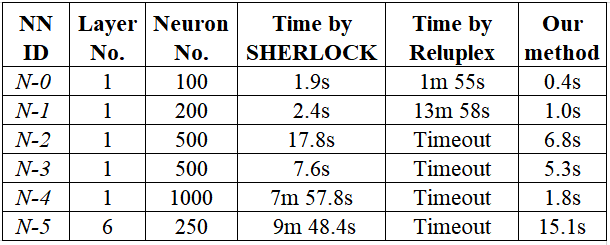
\includegraphics[width=0.9\linewidth]{images/robustnessVerification/f2.png}
% 	\caption{Comparison with SHERLOCK and Reluplex}
% 	\label{fig-2}
% \end{figure}

% \begin{figure*}[ht]
% 	\begin{minipage}{0.46\linewidth}
% 	\centering
% 	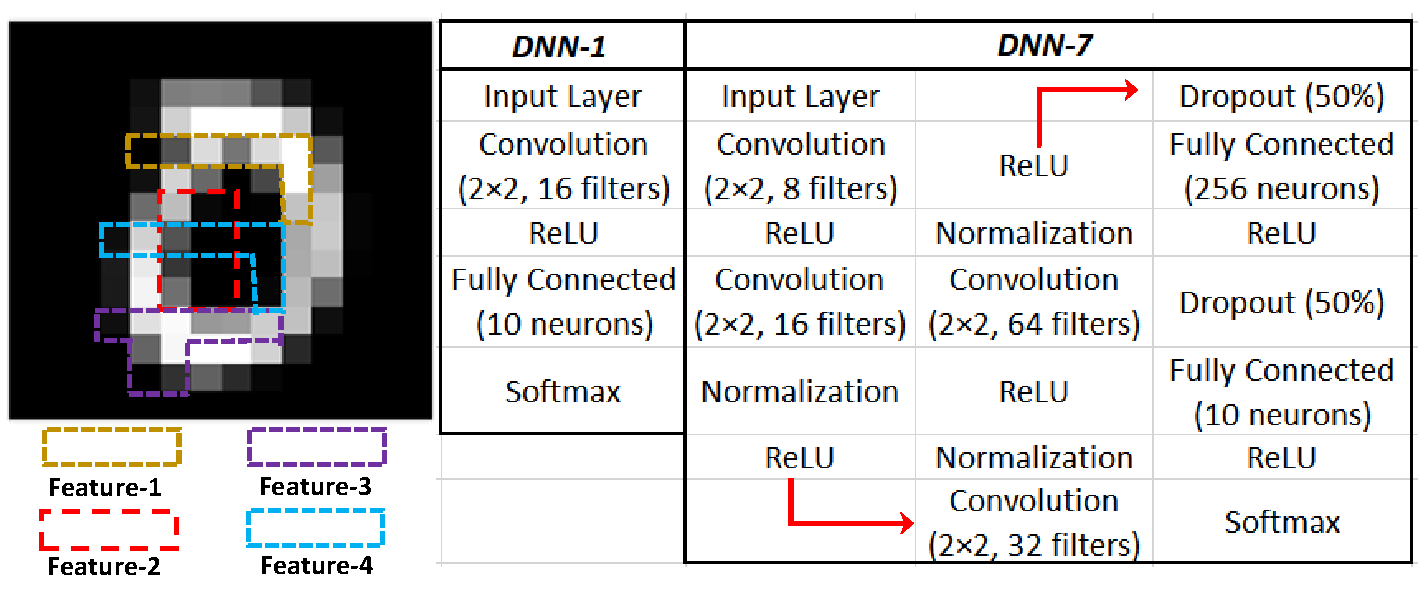
\includegraphics[width=1\linewidth]{images/robustnessVerification/f4.pdf}
% 	\subcaption{}
% 		\end{minipage}
% 		\begin{minipage}{0.54\linewidth}
% 		\centering
% 	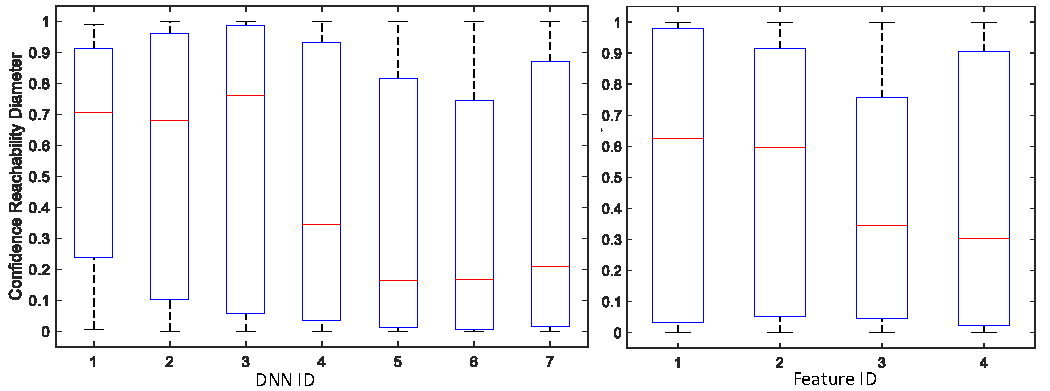
\includegraphics[width=1\linewidth]{images/robustnessVerification/f8.pdf}
% 		\subcaption{}
% 		\end{minipage}
% 			\vspace{-1pt}
% 			\caption{(a) The four features and the architecture of DNN-1 and DNN-7. (b) Left: boxplots of confidence reachability diameters for 7 DNNs, based on $4\times20$ analyses of each DNN. Right: boxplot of confidence reachability diameters for 4 features, based on $7\times20$ analyses of each feature. The red line represents the median value: a lower value indicates a more robust model or feature.}
% 	\label{fig-3}
% \end{figure*}

% \begin{figure*}[t]
% 	\begin{minipage}{0.32\linewidth}
% 	\centering
% 	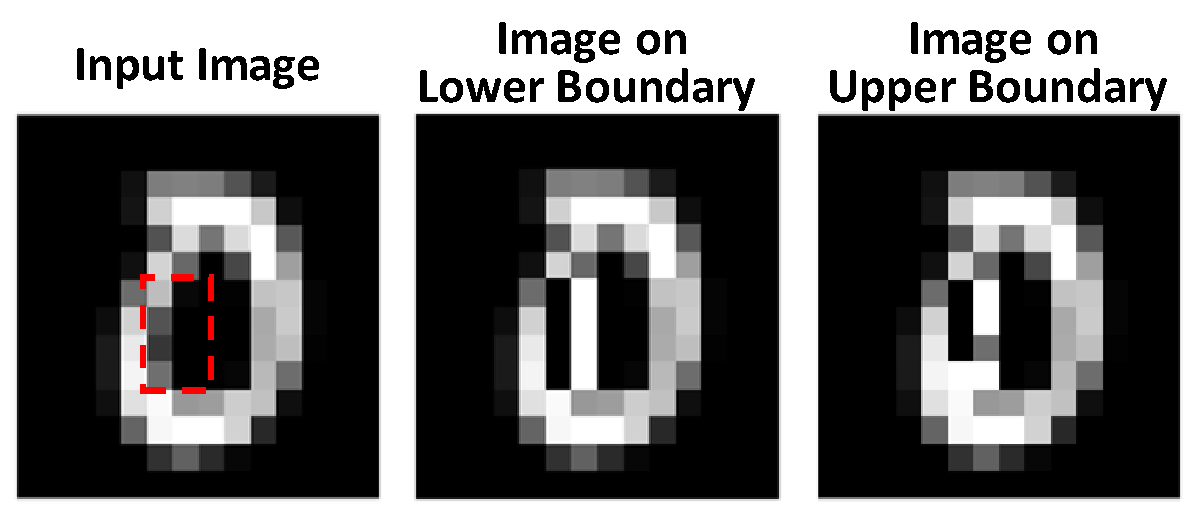
\includegraphics[width=0.9\linewidth]{images/robustnessVerification/f3.pdf}
% 		\subcaption{}
% 	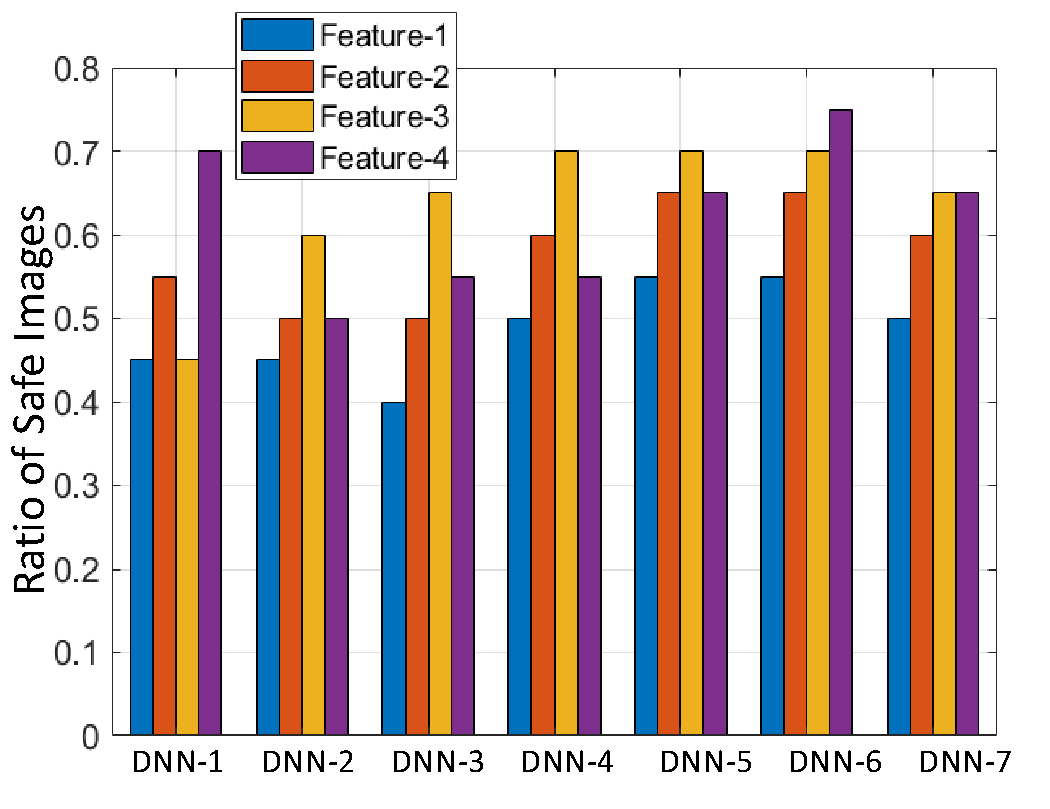
\includegraphics[width=1\linewidth]{images/robustnessVerification/f6.pdf}
% 	\subcaption{}
% 		\end{minipage}
% 		\begin{minipage}{0.68\linewidth}
% 		\centering
% 	\centering
% 	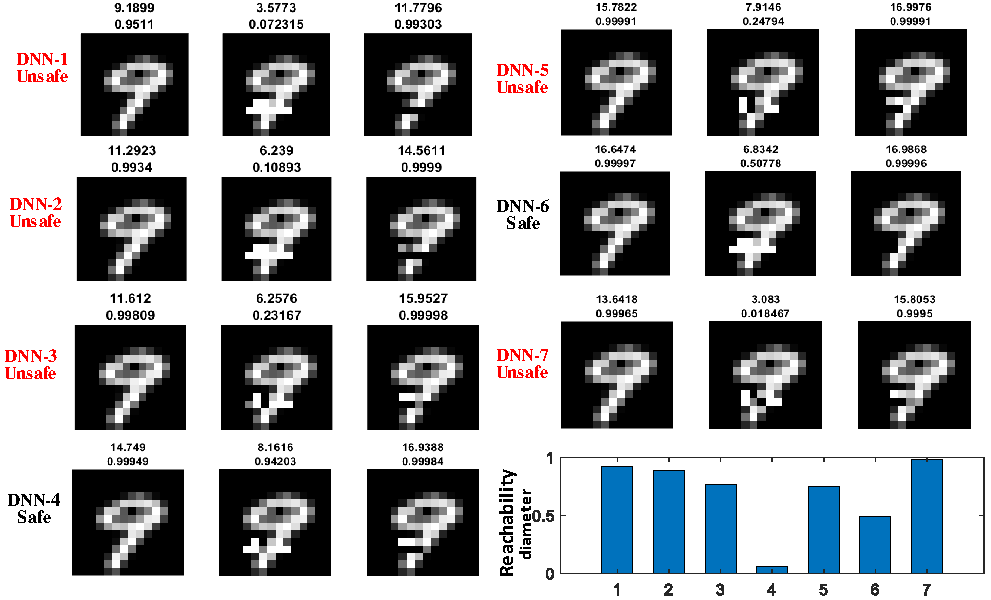
\includegraphics[width=1\linewidth]{images/robustnessVerification/f7.pdf}
% 	\subcaption{}
% 		\end{minipage}
% 			\caption{(a) Left: an original image (logit is 11.806, confidence of output being `0' is 99.95\%), where area marked by dashed line is the feature. Middle: an image on the confidence lower bound. Right: an image on the confidence upper bound; for the output label `0', the feature's output range is $[74.36\%,99.98\%]$, and logit reachability is $[7.007, 13.403]$. (b) Ratios of safe images for 7 DNNs and 4 features. (c) A detailed example comparing the safety and robustness of DNNs for image '9' and Feature-3: the top number in the caption of each figure is logit and the bottom one is confidence; the unsafe cases are all misclassified as `8'; the last bar chart shows their confidence reachability diameters.}
% 	\label{fig-4}
% \end{figure*}
 

% \subsection{Case Study One: Safety Verification}

% We use our tool to conduct logit and output range analysis.
% %for verifying the safety of deep neural networks, and compare robustness of different networks and input subspaces. 
% Seven convolutional neural networks, represented as DNN-1,...,DNN-7, were trained on the MNIST dataset. Images are resized into $14\times 14$ to enforce that a DNN with deeper layers tends to over-fit. The networks have different layer types, including ReLu, dropout and normalization, and the number of layers ranges from $5$ to $19$. Testing accuracies range from $95\%$ to $99\%$, and $\epsilon=0.05$ is used in our experiments.

% We randomly choose 20 images (2 images per label) and manually choose 4 features
% %\footnote{We also conduct experiments in which features are selected by object detection techniques such as SIFT \cite{Lowe1999}. We cannot include the results for space limit, but the conclusions are similar. } 
% such that each feature contains 8 pixels, i.e., $X'=[0,1]^8$. Fig.~\ref{fig-3} (a) illustrates the four features and the architecture of two DNNs with the shallowest and deepest layers, \ie~DNN-1 and DNN-7. 

% \vspace{1mm}

% \noindent{\bf Safety Verification}
% %
% %Then we conduct the reachability analysis for those features. 
% Fig.~\ref{fig-4} (a) shows an example: for DNN-1, Feature-4 is \emph{guaranteed to be safe} with respect to the image $x$ and the input subspace $X'$.
% %to any adversarial perturbation. 
% Specifically, the reachability interval is $R(\Pi_0,X',\epsilon) = [74.36\%,99.98\%]$, which means that $l(\Pi_0,X',\epsilon)=74.36\%$. By this, we have $u(\oplus_{-0},X',\epsilon) \leq (1-0.7436) < 0.7436 = l(\Pi_0,X',\epsilon)$. Then, by Theorem \ref{thm:safety}, we have 
% $\Safe(\text{DNN-1},x,X')$. Intuitively, no matter how we manipulate this feature, the worst case is to reduce the confidence of output being `0' from 99.95\% (its original confidence probability) to 74.36\%. 


% \subsection{Case Study Two: Statistical Quantification of Robustness}


% \noindent{\bf Statistical Comparison of Safety}
% %
% Fig.~\ref{fig-4} (b) compares the ratios of safe images for different DNNs and features. It shows that: \one~no DNN is 100\% safe on those features: DNN-6 is the safest one and DNN-1, DNN-2 and DNN-3 are less safe, which means a DNN with well chosen layers are safer than those DNNs with very shallow or deeper layers; and \two~the safety performance of different DNNs is consistent for the same feature, which suggests that the feature matters -- some features are easily perturbed to yield adversarial examples, e.g., Feature-1 and Feature-2.

% \vspace{1mm}

% \noindent{\bf Statistical Comparison of Robustness}
% %
% Fig.~\ref{fig-3} (b) compares the robustness of networks and features with two boxplots over the reachability diameters, where the function $o$ is $\Pi_j$ for a suitable $j$. We can see that DNN-6 and DNN-5 are the two most robust, while DNN-1, DNN-2 and DNN-3 are less robust. Moreover, Feature-1 and Feature-2 are less robust than Feature-3 and Feature-4. 

% %Together with the above, we can see that 
% We have thus demonstrated that
% reachability analysis with our tool can be used to quantify the safety and robustness of deep learning models. In the following, we perform a comparison of networks over a fixed feature. 

% \vspace{1mm}

\subsection{A Running Numerical Example}

In this section, we will use a numerical example to illustrate the fundamental differences between the reachability analysis method, DeepGO, constraint-solver based approach~\cite{bunel2017piecewise,CNR2017,ehlers2017formal1}, and $AI^2$ - a verification method based Abstract Interpretation (AI)~\cite{gehr2018ai21}.

Fig.~\ref{fig-E2} shows the details of a neural network we used for investigation. This toy neural network has two input $x_1$ and $x_2$, two output $y_1$ and $y_2$. It contains one hidden layer with ReLU activation functions. We denote the ReLU activation by two parts: one part is $r_1$ and $r_1$ denoting the values before the activation, another part is $h_1$ and $h_2$ representing the values after activation. In this numerical example, we aim to solve the following reachability problem.

\begin{problem}\label{problem-E1}
{\em Given a neural network and the box-constraints on its inputs, i.e., $x_1\in [4,6], x_2 \in [4.5,5]$, what is the output range of $y_1$?}
\end{problem}

We will first show constraint-solver based solution, then reveal how $AI^2$ works and finally show how to use DeepGO to solve this problem.
 
\begin{figure}[t]
	\centering
	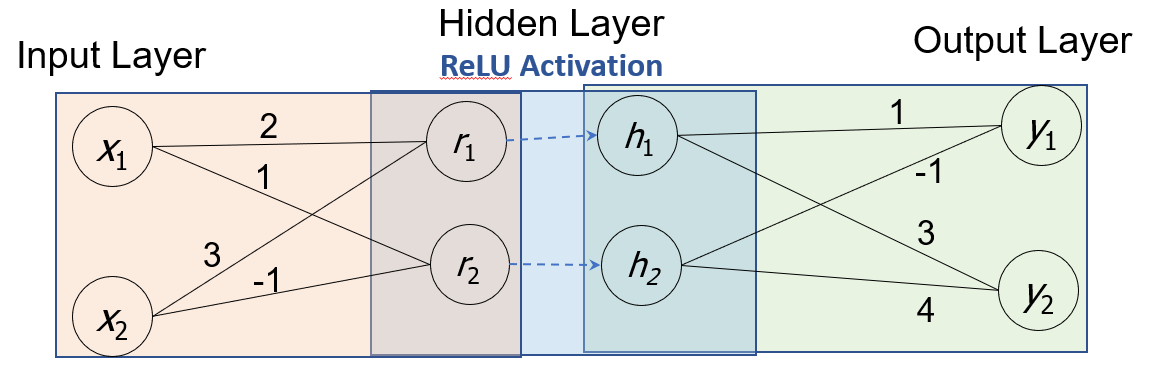
\includegraphics[width=0.85\linewidth]{images/robustnessVerification/Capture5.PNG}
	\caption{Encoding the whole neural network layer by layer on a neural networks with one ReLU-based hidden layer}
	\label{fig-E2}
\end{figure}
  
\subsubsection{Constraint-Solver based Approach}

As discussed in previous chapters, the majority of the solutions to solve Problem~\ref{problem-E1} are based on MILP or LP solvers, including SHERLOCK~\cite{dutta2017output}, Reluplex~\cite{katz2017reluplex}, Planet~\cite{ehlers2017formal1}, MIP~\cite{CNR2017} and BaB~\cite{bunel2017piecewise}, etc. We will reveal the basic idea of those works by using an LP-based solver as an example.

The first step is to encode the input and neural networks. As shown in Fig.~\ref{fig-E2}, we can encode the whole neural network layer by layer.

\begin{equation}\label{eqn-encode}
    \begin{split}
        \begin{cases}
        r_1 = 2x_1 + 3x_2\\
        r_2 = x_1 - x_2\\
        h_1 = \begin{cases}
    r_1, & \text{if $r_1\geq 0$}.\\
    0, & \text{otherwise}.
  \end{cases}\\
  h_2 = \begin{cases}
    r_2, & \text{if $r_2\geq 0$}.\\
    0, & \text{otherwise}.
  \end{cases}\\
  y_1 = h_1 - h_2\\
  y_2 = 3h_1 - 4h_2\\
  4 \leq x_1 \leq 6\\
  4.5 \leq x_2 \leq 5
  \end{cases}
    \end{split}
\end{equation}

Then, to estimate the reachable interval of $y_1$, we also need to incorporate the target problem and formulate them into {\em four} linear programming problems based on the activation patterns of hidden neurons, as shown by the below equation.

\begin{equation}\label{eqn-encode}
    \begin{split}
       & \begin{cases}
        \max/\min~~y_1 = x_1 +4x_2\\
        \text{s.t.} \quad  2x_1 + 3x_2\geq 0\\
        \qquad x_1 - x_2 \geq 0\\
        \qquad 4\leq x_1 \leq 6\\
        \qquad 4.5\leq x_1 \leq 5\\
  \end{cases} 
  \bigcup  
        \begin{cases}
        \max/\min~~y_1 = 2x_1 +3x_2\\
        \text{s.t.} \quad  2x_1 + 3x_2\geq 0\\
        \qquad x_1 - x_2 \leq 0\\
        \qquad 4\leq x_1 \leq 6\\
        \qquad 4.5\leq x_1 \leq 5\\
  \end{cases}\\
  \bigcup &
  \begin{cases}
        \max/\min~~y_1 = -x_1 +x_2\\
        \text{s.t.} \quad  2x_1 + 3x_2\leq 0\\
        \qquad x_1 - x_2 \geq 0\\
        \qquad 4\leq x_1 \leq 6\\
        \qquad 4.5\leq x_1 \leq 5\\
  \end{cases}
    \bigcup
  \begin{cases}
        \max/\min~~y_1 = 0\\
        \text{s.t.} \quad  2x_1 + 3x_2\leq 0\\
        \qquad x_1 - x_2 \leq 0\\
        \qquad 4\leq x_1 \leq 6\\
        \qquad 4.5\leq x_1 \leq 5\\
  \end{cases}
    \end{split}
\end{equation}

By solving the above four linear programming problems using an LP solver, we can solve Problem~\ref{problem-E1} and calculate its reachable confidence interval $[21.5, 26]$.

\subsubsection{Abstract Interpretation based Approach}

A well-established verification work using Abstract Interpretation is $AI^2$~\cite{gehr2018ai21}. It phrases the problem of certifying neural networks in the classic abstract interpretation framework. The key ingredient in $AI^2$ is the layer-by-layer over-approximation of the neural network using zonotope-based abstract interpretation. 

Fig.~\ref{fig-E11} depicts the procedure of layer-by-layer zonotope abstract interpretation in $AI^2$ for solving Problem~\ref{problem-E1}. $AI^2$ first adopts a zonotope to abstract all the inputs. 
%
\begin{equation}
    \begin{split}
        \mathbf{Z}_1 = \{(x_1,x_2)~|~x_1 = a_1 +5; x_2= 0.25a_2 +4.75\}
    \end{split}
\end{equation}
%
where $a_1 \in [-1,1]$ and $a_2 \in [-1,1]$.

Then it performs the zonotope abstract transformation based on the affine transformation from the input layer into the pre-activation layer. Please note that affine transformation is exact in zonotope-based abstraction.
%
\begin{equation}
    \begin{split}
        \mathbf{Z}_2 = \{(r_1,r_2)~|~r_1 = 24.25+2a_1+0.75a_2; r_2= 0.25 + a_1 - 0.25a_2\}
    \end{split}
\end{equation}
%
where $a_1 \in [-1,1]$ and $a_2 \in [-1,1]$.


\begin{figure}[t]
	\centering
	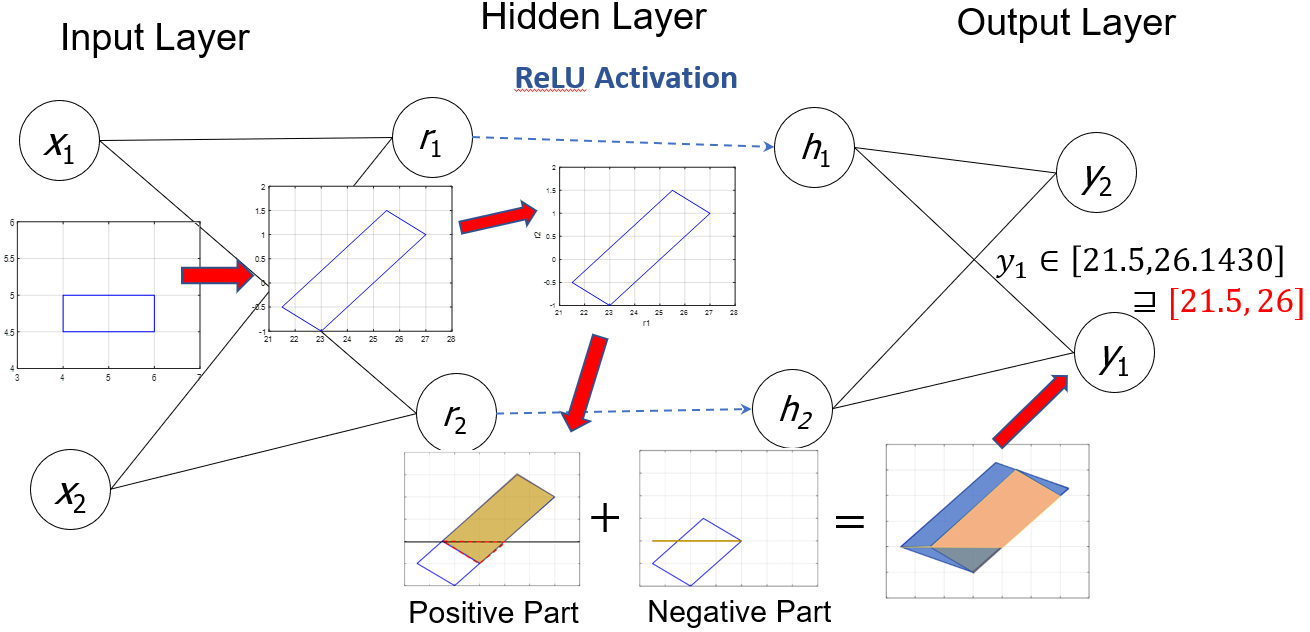
\includegraphics[width=1\linewidth]{images/robustnessVerification/Capture8.PNG}
	\caption{Illustration of layer-by-layer over-approximation using zonotope abstract interpretation in $AI^2$}
	\label{fig-E11}
\end{figure}

Next, $AI^2$ considers the zonotope over-approximation on the first ReLU hidden neuron. Since $r_1\geq 0$ always holds, zonohedron $\mathbf{Z}_2$ will transfer into the next layer without over-approximation loss. Thus we have $\mathbf{Z}_3 = \mathbf{Z}_2$. However, for the second ReLU hidden neuron, the zonotope abstraction is complicated since $r_2$ is partially negative and partially positive, which requires two cases:

\begin{itemize}
    \item Zonotope Over-approximation on Positive Part: As shown in Figure~\ref{fig-E11}, the positive part $\mathbf{Z}_3\cap \{r_2\geq 0\}$ is not a zonohedron. So we perform the zonotope over-approximation and get a new zonohedron:
    $$\mathbf{Z}_{4,p} = \{(h_1,h_2)~|~h_1 = 24.75+1.5a_1+0.75a_2; h_2= 0.5 + 0.75a_1 - 0.25a_2\}$$
    
     \item Zonotope Over-approximation on Negative Part: Similarly, we get a new zonotope 
    $$\mathbf{Z}_{4,n} = \{(h_1,h_2)~|~h_1 = 23.25+0.75a_1+a_2; r_2 = 0\}$$
\end{itemize}

Then, as shown in Fig.~\ref{fig-E11}, we perform a joint on two zonotopes $\mathbf{Z}_{4,p}\cup \mathbf{Z}_{4,n}$, and perform another zonotope over-approximation:
%
\begin{equation}
    \mathbf{Z}_5 = \{(h_1,h_2)~|~h_1 = 24.3929+1.6429a_1+1.25a_2; h_2= 0.5714 + 0.8214a_1 - 0.25a_2\}
\end{equation}
%
where $a_1 \in [-1,1]$ and $a_2 \in [-1,1]$.


Finally, we can get the symbolic express on $y_1$ based on the affine transformation from after-activation layer to output layer:
\begin{equation}
    y_1 = h1 - h2 = 23.8215 + 0.8215a_1 - 1.5a_2
\end{equation}
where $a_1 \in [-1,1]$ and $a_2 \in [-1,1]$. Thus, using $AI^2$, we can get the reachable output of $y_1$ is $[21.5, 26.1430] \supseteq	[21.5, 26]$, which is an over-approximation of the actual reachable state of the neural network. As illustrated by Fig.~\ref{fig-E12}, the yellow area is the actual information passed into the output layer, and the blue area is the over-approximation loss brought by the layer-by-layer zonotope abstractions.

\begin{figure}[t]
	\centering
	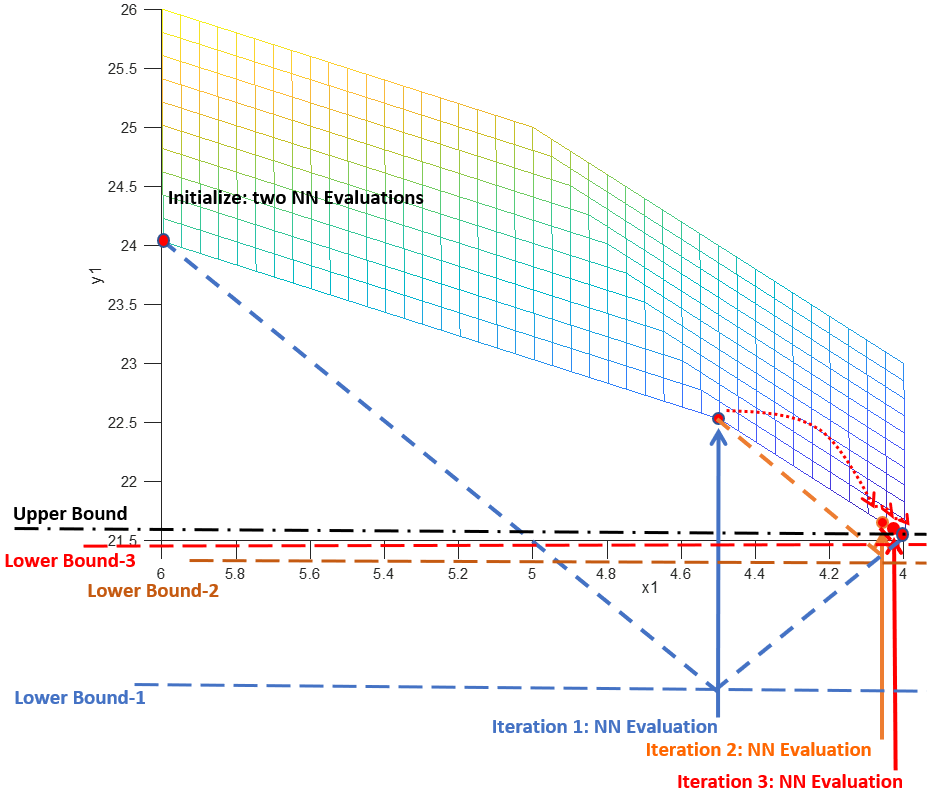
\includegraphics[width=0.9\linewidth]{images/robustnessVerification/Capture10.PNG}
	\caption{Illustration of working mechanism of DeepGO for solving the reachability problem}
	\label{fig-E13}
\end{figure}
  

\subsubsection{Reachability Analysis by DeepGO}


Now we show how DeepGO solve this reachability problem. As we can prove the target neural network in Fig.~\ref{fig-1} is proved to be Lipschitz continuous~\cite{szegedy2014intriguing,RHK2018}, to solve Problem~\ref{problem-E1}, it can be reduced to solve the following minimisation problems.
\begin{equation}\label{eqn-deepagn}
   \begin{cases}
        \min_{x_1,x_2}~~y_1 = f(x_1,x_2)\\
        \text{s.t.} \quad 4\leq x_1 \leq 6\\
        \qquad 4.5\leq x_1 \leq 5\\
  \end{cases}
\end{equation}

By solving the above two problems, we can get the reachable value of $y_1$. Fig.~\ref{fig-E13} illustrates the optimisation procedure of DeepGO iteration by iteration\footnote{For visualisation, we just show the $x_1$ dimension.}.

\begin{itemize}
    \item Initialisation: It evaluates two ending points on $x_1$: 4 and 6, and gets the Upper Bound-1 and Lower Bound-1.
    \item Iterations: DeepGO then evaluates $y_1$ on the point of Lower Bound-1, and refines the lower bound to get Lower Bound-2 (described in Section~\ref{sec:onedimensional}). Similarly, we continue the optimisation iterations and get a series of lower bounds.
    \item Termination: After the gap between lower bound and upper bound is close enough, i.e., smaller than a positive number $\epsilon = 0.0001$, we stop and return the value of $y_1^* = 21.5$, which is the lowest value that the neural network can reach in Problem~\ref{problem-E1}.
\end{itemize}

To get the largest reachable value, We replace objective function in Eqn.~\ref{eqn-deepagn} by $y_1 = - f(x_1,x_2)$ and perform the same procedure to get $y_1^{**} = 26$. By DeepGO, we can finally get the reachable interval of the neural network: $y_1 = [21.5, 26]$. 

\begin{figure}[t]
	\centering
	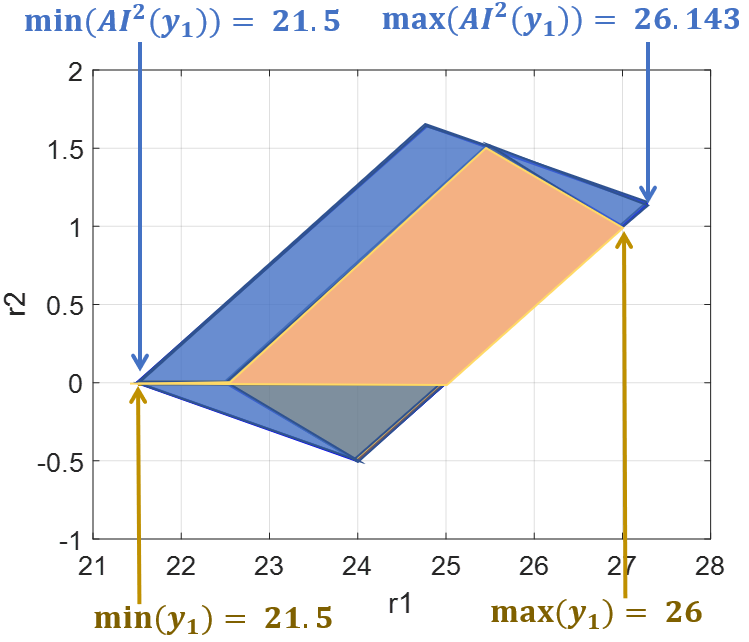
\includegraphics[width=0.55\linewidth]{images/robustnessVerification/Capture9.PNG}
	\caption{The comparison between $AI^2$ and DeepGO in terms of over-approximation error}
	\label{fig-E12}
\end{figure}

In summary, for Problem~\ref{problem-E1}, as we can see from Fig.~\ref{fig-E12}, DeepGO can calculate the reachable range of the neural network without an over-approximation error, but $AI^2$ brings a non-trivial error due to its over-approximation nature from the abstract interpretation. On the other hand, although LP/MILP based solution can also obtain an exact reachable range, DeepGO is much more efficient, especially for a neural network with a massive number of neurons.

%\subsection{Conclusion}

%This chapter introduces a reachability analysis method for deep neural networks, called DeepGO. It has provable guarantees and can be applied to neural networks with deep layers and nonlinear activation functions. The numerical example demonstrates the merits of this approach, which marks an important step towards a practical, guaranteed safety verification for DNNs.




% \chapter{Robustness Verification via Reachability Analysis}\label{chap:reachabilityAnalysis}

% Concerns have been raised about the suitability of deep neural networks (DNNs), or systems with DNN components, for deployment in safety-critical applications, see e.g., \cite{AOSCSM2016}. To ease this concern and gain users' trust, DNNs need to be certified similarly to %software and hardware   
% systems such as airplanes and automobiles. In this paper, we propose to study a generic reachability problem which, for a given DNN, an input subspace and a function over the outputs of the network, computes the upper and lower bounds over the values of the function. The function is generic, with the only requirement that it is Lipschitz continuous. %and has the DNN's output as its input. 
% We argue that this problem is fundamental for certification of DNNs, %can be a core problem towards certifying DNNs 
% as it can be instantiated into several key correctness problems, including adversarial example generation \cite{szegedy2014intriguing,GSS2014}, safety verification \cite{HKWW2017,katz2017reluplex,RWSHKK2018}, output range analysis \cite{LM2017,dutta2017output}, and robustness comparison. 


% %$R_j(X')$ for a given class label $j\in [1..m]$.
% % is the set of possible confidence levels $c_j(x)$ over the label $j$. 
% % An error bound may be needed for practical reasons. 
% To certify a system, a certification approach needs to provide not only a result but also a guarantee over the result, such as the error bounds. 
% Existing approaches for analysing DNNs with a guarantee work by either reducing the problem to a constraint satisfaction problem that can be solved by MILP \cite{LM2017,CNR2017,bunel2017piecewise,xiang2017output}, SAT \cite{NKPSW2017} or SMT \cite{katz2017reluplex,bunel2017piecewise} techniques, or applying search algorithms over discretised vector spaces \cite{HKWW2017,wicker2018feature}. Even though they are able to achieve guarantees, they suffer from two major weaknesses. Firstly, their subjects of study are restricted. 
% More specifically, they can only work with layers conducting linear transformations (such as convolutional and fully-connected layers) and simple non-linear transformations (such as ReLU), and cannot work with other important layers, such as the sigmoid, max pooling and softmax layers that are widely used in state-of-the-art networks. Secondly, the scalability of the constraint-based approaches is significantly limited by both the capability of the solvers and the size of the network, and they can only work with networks with a few hundreds of hidden neurons. However, state-of-the-art networks usually have millions, or even billions, of hidden neurons. 

% This paper proposes a novel approach to tackle the generic reachability problem, which does not suffer from the above weaknesses and provides provable guarantees %over its results 
% in terms of the upper and lower bounds over the errors. The approach is inspired by recent advances made in the area of global optimisation~\cite{gergel2016adaptive,grishagin2018convergence}. 
% For the input subspace defined over a set of input dimensions, an adaptive nested optimisation algorithm is developed. The performance of our algorithm is not dependent on the size of the network and it can therefore scale to work with large networks. 

% Our algorithm assumes certain knowledge about the DNN. However, instead of directly translating the activation functions and their parameters (i.e., weights and bias) into linear constraints, % as done in the reduction approaches, 
% it needs a Lipschitz constant of the network. For this, we show that several layers that cannot be directly translated into linear constraints are actually Lipschitz continuous, and we are able to compute a tight Lipschitz constant by analysing the activation functions and their parameters. 

% We develop a software tool DeepGO\footnote{Available on \url{https://github.com/trustAI/DeepGO}.} and evaluate its performance by comparing with existing constraint-based approaches, namely, SHERLOCK \cite{dutta2017output} and Reluplex \cite{katz2017reluplex}. We also demonstrate % on several problems that can be handled by them. Our experiments include those networks that cannot be handled by existing algorithms. 
% our tool on DNNs that are beyond the capability of existing tools.

% %Practically, the layer-to-layer mapping functions can be various types of activation functions such as ReLU, Leaky ReLU, sigmoid function, Hyperbolic tangent function etc., or different pooling operations such as max pooling and contrast-normalization pooling, and softmax layer (usually in the last layer). Noted that existing methods of reachability analysis for DNNs are all based on MLP [?], SAT [?] or SMT [?] techniques, which enable them has the following three major limitations: \one~they are only workable on the ReLU activation functions due to the linearizion formulation; \two~they cannot analyses softmax layer which enables their reachability analysis not complete; and \three~those methods are based on a layer-by-layer analysis which makes them only workable for a small-scale neural network(such as 3-layer NN with only hundreds of neurons. 

% %To deal with the above limitation, in this paper, we tackle the problem from a "black-box" point of view, which is neither depends on the layer-by-layer analysis nor built upon any MLP solvers. The only assumption we rely on is that the targeted deep neural network satisfies the Lipschitz continuity assumption.
% 		%\vspace{1mm}

% %\vspace{-3pt}

% \section{Lipschitz Continuity of Deep Learning}\label{sec:lipschitz}

% This section shows that feed-forward DNNs are Lipschitz continuous.
% %and presents an approach to compute, for a given DNN, its Lipschitz constant. 
% %
% %preliminaries and mathematical problem formulations.
% %
% %\subsection{Preliminaries}
% %
% %
% %Let $N$ be a network with a set $C$ of classes. Given an input $\inputImage$ and a class $c \in C$, we use $N(\inputImage,c)$ to denote the confidence (expressed as a probability value obtained from normalising the score) of $N$ believing that $\inputImage$ is in class $c$. Moreover, we write $N(\inputImage) = \arg\max_{c\in C} N(\inputImage,c)$ for the class into which $N$ classifies $\inputImage$. 
% %%z_Allsorted(1,end)
% %For our discussion of image classification networks, the input domain $\inputdomain$ is a vector space, which in most cases can be represented as 
% %%the pixel domain (i.e. all possible values a single pixel in an image can take on). For many images, the pixel domain is an alias for 
% %${\rm I\!R_{[0,255]}^{w\times h\times ch}}$, where $w,h,ch$ are the width, height, and number of channels of an image, respectively, and we let $P_0 = w\times h\times ch$ be the set of input dimensions. In the following, we may refer to an element in $w\times h$ as a pixel and an element in $P_0$ as a dimension. 
% %
% %This paper focuses on the confidence reachability analysis of a multi-layer feed-forward neural networks. 
% Let $f: \mathbb{R}^n \rightarrow \mathbb{R}^m$ be a $N$-layer 
% %feed-forward neural 
% network such that, for a given input $x\in \mathbb{R}^n$, $f(x) = \{c_1,c_2,...,c_m\}\in \mathbb{R}^m$ represents the confidence values for $m$ classification labels. Specifically, we have 
% $	f(x) = f_N(f_{N-1}(...f_1(x;W_1,b_1);W_2,b_2);...);W_N,b_N)
% $ where $W_i$ and $b_i$ for $i = 1,2,...,N$ are learnable parameters and $f_i(z_{i-1};W_{i-1},b_{i-1})$ is the function mapping from the output of layer $i-1$ to the output of layer $i$ such that $z_{i-1}$ is the output of layer $i-1$. Without loss of generality, we normalise the input to lie $x\in [0,1]^n$. The output $f(x)$ is usually normalised to be in $[0,1]^m$ with a softmax layer. 
	


% \begin{definition}[Lipschitz Continuity]
% 	Given two metric spaces $(X, d_X)$ and $(Y, d_Y)$, where $d_X$ and $d_Y$ are the metrics on the sets $X$ and $Y$ respectively, a function $f: X\rightarrow Y$ is called {\em Lipschitz continuous} if there exists a real constant $K\geq0$ such that, for all $x_1, x_2 \in X$:
% 	\begin{equation}
% 	 d_Y(f(x_1), f(x_2)) \le K d_X(x_1, x_2).
% 	\end{equation}
% 	$K$ is called the {\em Lipschitz constant} for the function $f$. The smallest $K$ is called {\em the Best Lipschitz constant}, denoted as $K_{best}$.
% \end{definition}

% \cite{szegedy2014intriguing} show that deep neural networks with half-rectified layers (\ie~convolutional or fully connected layers with ReLU activation functions), max pooling and contrast-normalization layers are Lipschitz continuous. They prove that the upper bound of the Lipschitz constant can be estimated via the operator norm of learned parameters $W$.

% Next, we show that the softmax layer, sigmoid and Hyperbolic tangent activation functions also satisfy Lipschitz continuity. First we need the following lemma~\cite{sohrab2003basic}.

% \begin{mylemma}\label{theo-1}
% Let $f: \mathbb{R}^n \rightarrow \mathbb{R}^m$,	if $||\partial{f(x)}/\partial{x}|| \leq K$ for all $x \in [a, b]^n$, then $f$ is Lipschitz continuous on $[a, b]^n$ and $K$ is its Lipschitz constant, where $||*||$ represents a norm operator.
% \end{mylemma}


% Based on this lemma, we have the following theorem.

% \begin{theorem}
% Convolutional or fully connected layers with the sigmoid activation function $s(Wx+b)$, Hyperbolic tangent activation function $t(Wx+b)$, and softmax function $p(x)_j$ are Lipschitz continuous and their Lipschitz constants are $\dfrac{1}{2}\norm{W}$, $\norm{W}$, and $\sup_{i,j}(\norm{x_i} + \norm{x_ix_j})$, respectively.
% \end{theorem}

% \begin{myproof}
% First of all, we show that the norm operators of their Jacobian matrices are bounded.

% (1)~Layer with sigmoid activation $s(q) = 1/(1+e^{-q})$ with $ q = Wx+b$:
% \begin{equation}
% \begin{split}
% \norm{\dfrac{\partial{s(x)}}{\partial{x}}} = \norm{\dfrac{\partial{s(q)}}{\partial{q}} \dfrac{\partial{q}}{\partial{x}}}
% \leq \norm{\dfrac{\partial{s(q)}}{\partial{q}}} \norm{\dfrac{\partial{q}}{\partial{x}}}\\
% \leq \norm{s(q)\circ(\mathbf{1}-s(q))}\norm{W}\leq \dfrac{1}{4}\norm{W}
% \end{split}
% \end{equation}

% (2)~Layer with Hyperbolic tangent activation function $t(q) = 2/(1+e^{-2q})-1$ with $ q = Wx+b$:
% \begin{equation}
% \begin{split}
% \norm{\dfrac{\partial{t(x)}}{\partial{x}}} = \norm{\dfrac{\partial{t(q)}}{\partial{q}} \dfrac{\partial{q}}{\partial{x}}}
% \leq \norm{\dfrac{\partial{t(q)}}{\partial{q}}} \norm{\dfrac{\partial{q}}{\partial{x}}}\\
% \leq \norm{\mathbf{1}-t(q)\circ t(q))}\norm{W}\leq \norm{W}
% \end{split}
% \end{equation}

% (3)~Layer with softmax function $p(x)_j = e^{x_j}/(\sum_{k = 1}^{n}{e^{x_k}})$ for $j = 1,...,m$ and $n = m$ (dimensions of input and output of softmax are the same):
% \begin{equation}
% \begin{split}
% \norm{\dfrac{\partial{p(x)_j}}{\partial{x_i}}} = 
% \left\{
% \begin{array}{ll}
% x_i(1-x_j), ~~i = j\\
% -x_ix_j,~~i\ne j
% \end{array}
% \right. \leq \sup_{i,j} (\norm{x_i} + \norm{x_ix_j})
% \end{split}
% \end{equation}
% Since the softmax layer is the last layer of a deep neural network, we can estimate its supremum based on Lipschitz constants of previous layers and box constraints of DNN's input.

% The final conclusion follows by Lemma 1 and the fact that all the layer functions are bounded on their Jacobian matrix. 
% \end{myproof}



% \section{Reachability Analysis of Deep Learning}


% %In this section, we present the formulate the problem of confidence reachability of a neural network. 
% Let $\obj: [0,1]^m \rightarrow \mathbb{R}$ be a Lipschitz continuous function statistically evaluating the outputs of the network. Our problem is to find its upper and lower bounds given the set $X'$ of inputs to the network. Because both the network $f$ and the %statistical evaluation 
% function $\obj$ are Lipschitz continuous, all values between the upper and lower bounds have a corresponding input, i.e., are reachable. 

% \begin{definition}[Reachability of Neural Network]
% Let $X'\subseteq [0,1]^n$ be an input subspace and $f: \mathbb{R}^n \rightarrow \mathbb{R}^m$ a network.
% % such that $f(x) = \{c_1,...,c_j,...,c_m\}\in [0,1]^m$ and $c_j$ is the $j$-th confidence output representing the probability of input $x$ belonging to $j$-th classification label. We also use $c_j(x)$ to represent the $j$-th output of DNN given input $x$. Then 
% The reachability of $f$ over the function $\obj$ under an error tolerance $\epsilon \geq 0$ is a set $R(\obj,X',\epsilon) = [l,u]$ such that 
% \begin{equation}
% \begin{split}
% \inf_{x' \in X'} \obj(f(x')) -\epsilon \leq l \leq \inf_{x' \in X'} \obj(f(x')) +\epsilon \\
% \sup_{x' \in X'} \obj(f(x')) - \epsilon \leq u \leq \sup_{x' \in X'} \obj(f(x')) + \epsilon.
% \end{split}
% \end{equation}
% We write $u(\obj,X',\epsilon)=u$ and $l(\obj,X',\epsilon)=l$ for the upper and lower bound, respectively. 
% %Confidence Upper Bound (CUB) and Confidence Lower Bound (CLB), respectively. 
% Then the reachability diameter is 
% 	\begin{equation}
%           D(\obj,X',\epsilon) =u(\obj,X',\epsilon)-l(\obj,X',\epsilon).
% 	\end{equation}
% Assuming these notations, we may write $D(\obj,X',\epsilon;f)$ if we need to explicitly refer to the network $f$. 
% \end{definition}

% In the following, we instantiate $\obj$ with a few concrete functions, and show that several key verification problems for DNNs can be reduced to our reachability problem. 

% \begin{definition}[Output Range Analysis]
% Given a class label $j\in [1,..,m]$, we let $\obj = \Pi_j$ such that $\Pi_j((c_1,...,c_m))=c_j$. 
% \end{definition}

% We write $c_j(x) = \Pi_j(f(x))$ for the network's confidence in classifying $x$ as label $j$. 
% Intuitively, output range \cite{dutta2017output} quantifies how a certain output of a deep neural network (\ie~classification probability of a certain label $j$) varies in response to a set of DNN inputs with an error tolerance $\epsilon$. Output range analysis can be easily generalised to logit \footnote{Logit output is the output of the layer before the softmax layer. The study of logit outputs is conducted in, e.g., \cite{PMJFCS2015,dutta2017output}.} range analysis.

% We show that the safety verification problem \cite{HKWW2017} can be reduced to solving the reachability problem. 

% \newcommand{\Safe}{{\tt S}}
% \newcommand{\Robust}{{\tt R}}

% \begin{definition}[Safety]
% A network $f$ is safe with respect to an input $x$ and an input subspace $X'\subseteq [0,1]^n$ with $x \in X'$, written as $\Safe(f,x,X')$, if 
% \begin{equation}
% \forall x' \in X': \arg\max_{j} c_j(x') = \arg\max_{j} c_j(x)
% \end{equation} 
% %where $c_j(x) = f(x)_j$ returns $N$'s confidence in classifying $x$ as label $j$. 
% \end{definition}

% We have the following reduction theorem. 

% %For the reduction, we define two functions $o_1=\Pi_j$ such that $j=\arg\max_{j}c_j(x)$, and $o_2 = +_{-j}$ such that $+_{-j}(c_1,...,c_m) = \sum_{i=1, i\neq j}^{m} c_i$. Therefore, we have 

% \begin{theorem}\label{thm:safety}
% A network $f$ is safe with respect to $x$ and $X'$ s.t. $x \in X'$ if and only if
% $u(\oplus,X',\epsilon) \leq 0$,
% %$l(\Pi_j,X',\epsilon) \geq u(\oplus_{-j},X',\epsilon)$
% where $\oplus(c_1,...,c_m) = \max_{i\in \{1..m\}}(\Pi_{i} (c_1,...,c_m) - \Pi_{j} (c_1,...,c_m))$ and $j=\arg\max_{j}c_j(x)$. The error bound of the safety decision problem by this reduction is $2\epsilon$. 
% \end{theorem}

% It is not hard to see that the adversarial example generation \cite{szegedy2014intriguing}, which is to find an input $x' \in X'$ such that $\arg\max_{j} c_j(x') \neq \arg\max_{j} c_j(x)$, is the dual problem of the safety problem. 

% The following two problems define the robustness comparisons between the networks and/or the inputs. 

% \begin{definition}[Robustness]
% Given two homogeneous\footnote{ Here, two networks are homogeneous if they are applied on the same classification task but may have different network architectures (layer numbers, layer types, etc) and/or parameters.}
% %E.g., two different neural networks but both are for the MNIST image classification task.} 
% networks $f$ and $g$, we say that $f$ is strictly more robust than $g$ with respect to a function $\obj$, an input subspace $X'$ and an error bound $\epsilon$, written as $\Robust_{o,X',\epsilon}(f,g)$, if $D(\obj,X',\epsilon;f) < D(\obj,X',\epsilon;g)$.

% %$j$-th output and an input subspace $\bar{x}$ if $D_j(\bar{x};f(x)) < D_j(\bar{x};g(x))$.
% \end{definition}

% \begin{definition}
% 	Given two input subspaces $X'$ and $X''$ and a network $f$, we say that $f$ is more robust on $X'$ than on $X''$ with respect to a statistical function $\obj$ and an error bound $\epsilon$, written as $\Robust_{f,o,\epsilon}(X',X'')$, if $D(\obj,X',\epsilon) < D(\obj,X'',\epsilon)$.
% %$D_j(\bar{x}) < D_j(\hat{x})$.
% \end{definition}

% Thus, by instantiating the function $\obj$, we can quantify the output/logit range of a network, evaluate whether a network is safe, and compare the robustness of two homogeneous networks or two input subspaces for a given network.
% 		%\vspace{-1mm}

% %\vspace{-3pt}
% \subsection{Confidence Reachability with Guarantees}
% %\vspace{-1pt}

% Section~\ref{sec:lipschitz} shows that a trained deep neural network is Lipschitz continuous regardless of its layer depth, activation functions and number of neurons. Now, to solve the reachability problem, we need to find the \emph{global} minimum and maximum values given an input subspace, assuming that we have a Lipschitz constant $K$ for the function $o\!\cdot\!f$. In the following, we let $\of = o\!\cdot\!f$ be the concatenated function. Without loss of generality, we assume the input space $X'$ is a box-constraint, which is clearly feasible since images are usually normalized into $[0,1]^n$ before being fed into a neural network.

% % Thus we need to solve the following problem. Here we start to use $x$ instead of $\bar{x}$ (we can treat the fixed dimensions in input space as a learned parameters in neural network) and drop index $j$ (since we can perform the some analysis to each output separately). 
% The computation of the minimum value is reduced to solving the following optimization problem with guaranteed convergence to the global minimum (the maximization problem can be transferred into a minimization problem):
% \begin{equation}\label{equ-8}
% \begin{split}
% \min\limits_{x}~~\of(x),~~~s.t.~~x \in [a,b]^n
% \end{split}
% \end{equation}
% However, the above problem is very difficult since $\of(x)$ is a highly non-convex function which cannot be guaranteed to reach the global minimum by regular optimization schemes based on gradient descent. Inspired by an idea from optimisation, see e.g., \cite{piyavskii1972algorithm,TZ1989}, we design another continuous function $h(x,y)$, which serves as a lower bound of the original function $\of(x)$. Specifically, we need 
% %This idea is also widely adopted in optimization community.
% \begin{equation}\label{equ-9}
% \begin{split}
% \forall x, y \in [a,b]^n,~ h(x,y) \leq \of(x)~~\text{and}~~h(x,x) = \of(x)
% \end{split}
% \end{equation}
% %
% Furthermore, for $i\geq 0$, we let $\mathcal{Y}_i = \{y_0,y_1,...,y_i\} $ be a finite set containing $i+1$ points from the input space $ [a, b]^n$, and let $\mathcal{Y}_i \subseteq \mathcal{Y}_k$ when $k>i$, then we can define a function
% $H(x;\mathcal{Y}_i) = \max_{y\in \mathcal{Y}_i } h(x,y)$
%  which satisfies the following relation:
% \begin{equation}
% H(x; \mathcal{Y}_i) < H(x; \mathcal{Y}_k)\leq %\inf_{x\in [a,b]^n}
% \of(x), \forall i < k
% \end{equation}

% We use $l_i = \inf_{x\in [a,b]^n} H(x;\mathcal{Y}_i)$ to denote the minimum value of $H(x;\mathcal{Y}_i)$ for $x\in [a,b]^n$. Then we have 
% %can get the following relation:
% \begin{equation}
% l_0< l_1< ... < l_{i-1}< l_i \leq \inf_{x\in [a,b]^n} \of(x)
% \end{equation}
% Similarly, we need a sequence of upper bounds $u_i$ to have 
% \begin{equation}\label{eqn-14}
% \begin{split}
% l_0< ... < l_i \leq \inf_{x\in [a,b]^n} \of(x)\leq u_i< ...< u_0
% \end{split}
% \end{equation}
% By Expression (\ref{eqn-14}), we can have the following:
% \begin{equation}\label{eqn-15}
% \begin{split}
% \lim\limits_{i\to \infty}l_i = \min_{x\in [a,b]^n} \of(x) \text{   and   }
% \lim\limits_{i\to \infty}(u_i - l_i) = 0
% \end{split}
% \end{equation}

% Therefore, we can asymptotically approach the global minimum. Practically, we execute a finite number of iterations by using an error tolerance $\epsilon$ to control the termination. 
% %
% %\begin{myremarks}
% %	Whenever terminated, it returns a lower bound and a upper bound of the global minimum, and we can evaluate the quality of global minimum obtained so far.
% %\end{myremarks}
% %
% In next sections, we present our approach, which constructs a sequence of lower and upper bounds, and show that it can converge with an error bound. To handle the high-dimensionality of DNNs, our approach is inspired by the idea of adaptive nested optimisation in \cite{gergel2016adaptive}, with significant differences in the detailed algorithm and convergence proof. 

% %We first discuss the one-dimension case and then the multiple-dimension case.
% \begin{figure}[t]
% 	\centering
% 	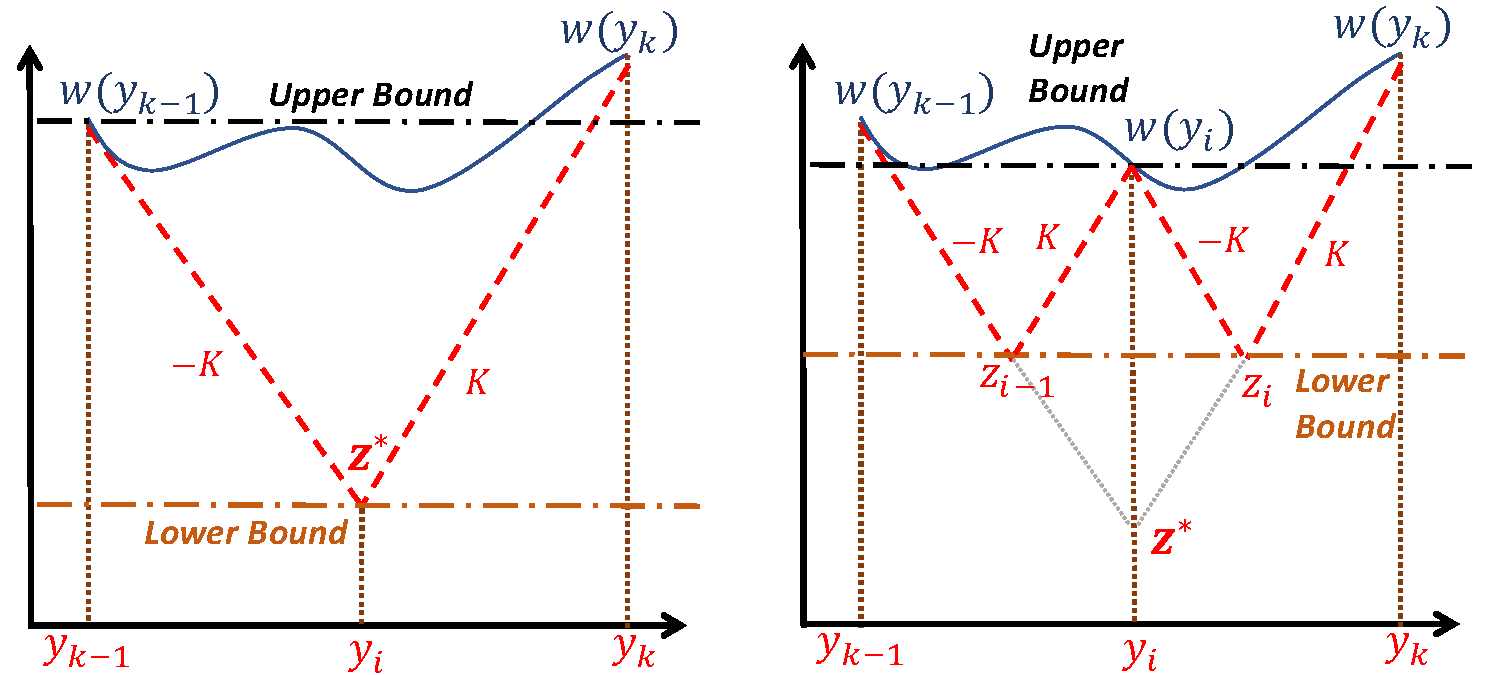
\includegraphics[width=1\linewidth]{images/robustnessVerification/f1.pdf}
% 	\caption{A lower-bound function designed via Lipschitz constant}
% 	\label{fig-1}
% \end{figure}


% \subsection{One-dimensional Case}\label{sec:onedimensional}


% We first introduce an algorithm which works over one dimension of the input, and therefore is able to handle the case of $x \in [a,b]$ in Eqn.~(\ref{equ-8}).
% %, based on Section 2 and Theorem~1, we can estimate the Lipschitz constants of a neural network numerically either or analytically. 
% The multi-dimensional optimisation algorithm will be discussed in Section~\ref{sec:multi} by utilising the one-dimensional algorithm. 

% We define the following lower-bound function.
% \begin{equation}\label{eqn-10}
% \begin{split}
% h(x,y) = \of(y) - K|x-y| \\
% H(x;\mathcal{Y}_i) = \max\limits_{y\in \mathcal{Y}_i }~~\of(y) - K|x-y|
% \end{split}
% \end{equation}
% where $K > K_{best}$ is a Lipschitz constant of $\of$ and $H(x;\mathcal{Y}_i)$ intuitively represents the lower-bound sawtooth function shown as Figure~1.
% %$L \geq K_{best}$ and we can estimate by $L = |d(c(x))/dx| + \eta$ $(\eta \geq 0)$ based on Theorem~1. 
% The set of points $\mathcal{Y}_i$ is constructed recursively. Assuming that, after $(i-1)$-th iteration, we have $\mathcal{Y}_{i-1} = \{y_0,y_1,..,y_{i-1}\}$, whose elements are in ascending order, and sets 
% $$
% \of(\mathcal{Y}_{i-1} )=\{\of(y_0), \of(y_1),..,\of(y_{i-1})\}
% $$
% $$\mathcal{L}_{i-1} = \{l_0,l_1,...,l_{i-1}\}$$
% $$\mathcal{U}_{i-1} = \{u_0,u_1,...,u_{i-1}\}$$
% $$\mathcal{Z}_{i-1} = \{z_1,...,z_{i-1}\}$$
% %where $z_{k} = \dfrac{\of(y_{k})+ \of(y_{k-1})}{2} - \dfrac{K(y_{k} - y_{k-1})}{2}, \forall k = 1,2,..,i-1$. 
% %
% The elements in sets $\of(\mathcal{Y}_{i-1} )$, $\mathcal{L}_{i-1}$ and $\mathcal{U}_{i-1}$ have been defined earlier. The set $\mathcal{Z}_{i-1}$ records the smallest values $z_k$ computed in an interval $[y_{k-1},y_k]$.

% In $i$-th iteration, we do the following sequentially:
% \begin{itemize}

% %\item Numerically estimate Lipschitz constant as $K = \eta \max_{j = 1,...,i-1} \{(\of(y_j) - \of(y_{j-1}))/(y_j - y_{j-1})\}$ where $\eta > 1$.

% 	\item Compute $y_i = \arg\inf_{x\in [a,b]} H(x;\mathcal{Y}_{i-1})$ as follows. Let $z^* = \min{\mathcal{Z}_{i-1} }$ and $k$ be the index of the interval $[y_{k-1},y_k]$ where $z^*$ is computed. Then we let 
% \begin{equation}\label{equ:newpoint}
% y_i = \dfrac{y_{k-1}+y_k}{2} - \dfrac{\of(y_{k}) - \of(y_{k-1})}{2K}
% \end{equation}

%  and have that $y_i \in (y_{k-1},y_k)$. 
	
% 	\item Let $\mathcal{Y}_i = \mathcal{Y}_{i-1}\cup\{y_i\}$, then reorder $\mathcal{Y}_i$ in ascending order, and update $\of(\mathcal{Y}_{i} )=\of(\mathcal{Y}_{i-1})\cup \{\of(y_i)\}$.
	
% 	\item Calculate 
% 	\begin{equation}\label{eqn-16}
% 	z_{i-1} = \dfrac{\of(y_{i})+ \of(y_{k-1})}{2} - \dfrac{K(y_{i} - y_{k-1})}{2}\end{equation}
	
% 	\begin{equation}\label{eqn-17}
% 	z_{i} = \dfrac{\of(y_{k})+ \of(y_{i})}{2} - \dfrac{K(y_{k} - y_{i})}{2}\end{equation} and update $\mathcal{Z}_{i} = (\mathcal{Z}_{i-1}\setminus \{z^*\}) \cup\{z_{i-1},z_{i}\} $.
	
% 	\item Calculate the new lower bound $l_i = \inf_{x\in [a,b]} H(x;\mathcal{Y}_i)$ by letting $l_i =\min\mathcal{Z}_{i}$,
% %\min \{l_{i-1}, z_{i-1},z_{i}\}$, 
% and updating $\mathcal{L}_{i} = \mathcal{L}_{i-1} \cup \{l_i \}$.
	
% 	\item Calculate the new upper bound $u_i = \min_{y\in \mathcal{Y}_i }\of(y)$ by letting $u_i = \min \{u_{i-1}, \of(y_i)\}$.
% \end{itemize}

% We terminate the iteration whenever $|u_i-l_i|\leq\epsilon$,
% % where $\epsilon$ is the error tolerance, 
% and let the global minimum value be $y^* = \min_{x\in [a,b]} H(x;\mathcal{Y}_{i})$ and the minimum objective function be $\of^* = \of(y^*)$. 

% Intuitively, as shown in Fig.~1, we iteratively generate lower bounds (by selecting in each iteration the lowest point in the saw-tooth function in the figure) by continuously refining a piecewise-linear lower bound function, which is guaranteed to below the original function due to Lipschitz continuity. The upper bound is the lowest evaluation value of the original function so far. 

% \subsection{Convergence Analysis}
% In the following, we show the convergence of this algorithm to the global minimum by proving the following conditions. 
% \begin{itemize}
%     \item Convergence Condition 1: $\lim\limits_{i\to \infty}l_i = \min\limits_{x\in [a,b]} \of(x)$
%     \item Convergence Condition 2: $\lim_{i\to \infty}(u_i - l_i) = 0$
% \end{itemize}

% \begin{myproof}[Monotonicity of Lower/Upper Bound Sequences]
% First, we prove that the lower bound sequence $\mathcal{L}_i$ is strictly monotonic. 
% 	Because 
% 	\begin{equation}l_i = \min \mathcal{Z}_i= \min \{(\mathcal{Z}_{i-1}\setminus \{z^*\}) \cup\{z_{i-1},z_{i}\} \} \end{equation} and $l_{i-1} = \min \mathcal{Z}_i$. To show that $l_i > l_{i-1}$, we need to prove $z_{i-1} > z^*$ and $z_{i} > z^*$. By the algorithm, $z^*$ is computed from interval $[y_{k-1}, y_k]$, so we have %
% 	\begin{equation}\label{eqn-19}
% 	z^* = \dfrac{\of(y_{k})+ \of(y_{k-1})}{2} - \dfrac{K(y_{k} - y_{k-1})}{2}\end{equation}
% 	We then have 
% 	\begin{equation}\label{equ:lowerbound}
% 	z_{i-1} - z^* = \dfrac{\of(y_i)-\of(y_k) - K(y_i - y_k)}{2}
% 	\end{equation} 
% 	Since $y_i < y_{k}$ and $K>K_{best}$, by Lipschitz continuity we have $z_{i-1} > z^* $. 
% 	Similarly, we can prove $z_{i} > z^* $. Thus $l_i > l_{i-1}$ is guaranteed. 
	
% 	Second, the monotonicity of upper bounds $u_i$ can be seen from the algorithm, since $u_i $ is updated to $ \min \{u_i, \of(y_i)\}$ in every iteration. 
% \label{proof2}
% \end{myproof}

% \begin{myproof}[Convergence Condition 1]
% 	~\\
% 	Since $\mathcal{Y}_{i-1}\subseteq \mathcal{Y}_{i}$, we have $H(x; \mathcal{Y}_{i-1}) \leq H(x; \mathcal{Y}_{i})$. Based on Proof~\ref{proof2}, we also have $l_{i-1}< l_i$. Then since  %And because 
% 	\begin{equation}l_i = \inf_{x\in [a,b]} H(x; \mathcal{Y}_{i}) \leq \min_{x\in [a,b]}\of(x)\end{equation} 
% 	the lower bound sequence $\{l_0,l_1,...,l_i\}$ is strictly monotonically increasing and bounded from above by $\min_{x\in [a,b]}\of(x)$. Thus $\lim_{i\to \infty}l_i = \min_{x\in [a,b]} \of(x)$ holds.
% \end{myproof}



% \begin{myproof}[Convergence Condition 2]
% 	~\\
% 	Since $\lim_{i\to \infty}l_i = \min_{x\in [a,b]} \of(x)$, we show $\lim_{i\to \infty}(u_i - l_i) = 0$ by showing that $\lim_{i\to \infty}u_i = \min_{x\in [a,b]} \of(x)$. 
% Since $\mathcal{Y}_{i} = \mathcal{Y}_{i-1} \cup\{y_i\}$ and $y_i \in X =[a, b]$, we have $\lim_{i\to \infty} \mathcal{Y}_{i} = X$. Then we have $\lim_{i\to \infty}u_i = \lim_{i\to \infty} \inf_{y\in \mathcal{Y}_i } \of(y) = \inf {\of(X)}$. Since $X = [a,b]$ is a closed interval, we can prove $\lim_{i\to \infty}u_i = \inf {\of(X)} = \min_{x\in [a,b]} \of(x)$. 
% \end{myproof}

% \subsection{Dynamically Improving the Lipschitz Constant}

% A Lipschitz constant closer to $K_{best}$ can greatly improve the speed of convergence of the algorithm. We design a practical approach to dynamically update the current Lipschitz constant according to the information obtained from the previous iteration: 
% \begin{equation}K = \eta \max_{j = 1,...,i-1} \abs{\dfrac{\of(y_j) - \of(y_{j-1})}{y_j - y_{j-1}}}\end{equation} where $\eta > 1$. We emphasise that, because 
% %during the iteration, we can numerically approximate the Lipschitz constant $K$, as we can show that 
% $$ \lim_{i \to \infty} \max_{j = 1,...,i-1} \eta\abs{\dfrac{\of(y_j) - \of(y_{j-1})}{y_j - y_{j-1}}} = \eta \sup_{y\in [a,b]} {\dfrac{d\of}{dy}} > K_{best}
% $$
% this dynamic update does not compromise the convergence.


% \subsection{Multi-dimensional Case}

% %We 
% %use the nested optimization approach, which is widely applied in optimization community~\cite{gergel2016adaptive}. Its core idea is to
% The basic idea is to decompose a multi-dimensional optimization problem into a sequence of nested one-dimensional subproblems. Then the minima of those one-dimensional minimization subproblems are back-propagated into the original dimension and the final global minimum is obtained. 
% \begin{equation}\label{equ-16}
% \min\limits_{x \in [a_i,b_i]^n}~~\of(x) =
% \min\limits_{x_1\in [a_1,b_1]}... \min\limits_{x_n\in [a_n,b_n]} \of(x_1,...,x_n)
% \end{equation}

% We first introduce the definition of $k$-th level subproblem.

% \begin{definition}\label{def:kthlevel}
% %[$k$-th Level Subproblem]
% 	The $k$-th level optimization subproblem, written as $\phi_k(x_1,...,x_k)$, is defined as follows: for $1\leq k \leq n-1$,
% 	%
% 	$$\phi_k(x_1,...,x_k) = \min_{x_{k+1}\in [a_{k+1},b_{k+1}]} \phi_{k+1}(x_1,...,x_k, x_{k+1}) $$
% 	%
% 	and for $k=n$, $$\phi_n(x_1,...,x_n) = \of(x_1,x_2,...,x_n).$$
% \end{definition}
% %
% Combining Expression (\ref{equ-16}) and Definition~\ref{def:kthlevel}, we have that $$\min_{{x} \in [a_i,b_i]^n}~~\of({x}) = \min_{x_1\in [a_1,b_1]} \phi_1(x_1)$$ which is actually a one-dimensional optimization problem and therefore can be solved by the method in Section~\ref{sec:onedimensional}. 

% However, when evaluating the objective function $\phi_1(x_1)$ at $x_1=a_1$, we need to project $a_1$ into the next one-dimensional subproblem $$\min_{x_2\in [a_2,b_2]}\phi_2(a_1,x_2)$$ We recursively perform the projection until we reach the $n$-th level one-dimensional subproblem, $$\min_{x_n\in [a_n,b_n]}\phi_n(a_1, a_2,..., a_{n-1},x_n)$$ 
% Once solved,
% % all one-dimension subproblems, 
% we back-propagate objective function values to the first-level $\phi_1(a_1)$ and continue searching from this level until the error bound is reached.

% \subsection{Convergence Analysis}

% We use mathematical induction to prove convergence for the multi-dimension case.
% %
% \begin{itemize}
% 	\item Base case: for all $ x\in \mathbb{R}$, $\lim_{i\to \infty}l_i = \inf_{x\in [a,b]} \of(x)$ and $\lim_{i\to \infty}(u_i - l_i) = 0$ hold.
	
% 	\item Inductive step: if, for all $ {x}\in \mathbb{R}^k$, $\lim_{i\to \infty}l_i = \inf_{{x}\in [a,b]^k} \of({x})$ and $\lim_{i\to \infty}(u_i - l_i) = 0$ are satisfied, then, for all $ {x}\in \mathbb{R}^{k+1}$, $\lim_{i\to \infty}l_i = \inf_{{x}\in [a,b]^{k+1}} \of({x})$ and $\lim_{i\to \infty}(u_i - l_i) = 0$ hold.
% \end{itemize}
% %
% The base case (\ie~one-dimensional case) is already proved in Section~\ref{sec:onedimensional}. Now we prove the inductive step. 



% \begin{myproof}
% 	By the nested optimization scheme, we have
% $$
% 	\min_{\mathbf{x} \in [a_i,b_i]^{k+1}}~~\of(\mathbf{x}) =\min_{x \in [a,b]}\Phi(x)
% 	$$
% 	$$
% 	\Phi(x) = \min_{\mathbf{y} \in [a_i,b_i]^k} \of(x,\mathbf{y})
% $$
% 	Since $\min_{\mathbf{y} \in [a_i,b_i]^k} \of(x,\mathbf{y})$ is bounded by an interval error $\epsilon_{\mathbf{y}}$, assuming $\Phi^*(x)$ is the accurate global minimum, then we have
% 	$$\Phi^*(x)-\epsilon_{\mathbf{y}}\leq \Phi(x) \leq \Phi^*(x)+\epsilon_{\mathbf{y}}$$ 
% 	So the $k+1$-dimensional problem is reduced to the one-dimensional problem %decomposed as problem 
% 	$\min_{x \in [a,b]}\Phi(x)$. The difference from the real one-dimensional case is that evaluation of $\Phi(x)$ is not accurate but bounded by $|\Phi(x) - \Phi^*(x)|\leq \epsilon_{\mathbf{y}}, \forall x \in [a,b]$, where $\Phi^*(x)$ is the accurate function evaluation.
	
% 	Assuming that the minimal value obtained from our method is $\Phi^*_{min} = \min_{x\in [a,b]} \Phi^*(x)$ under accurate function evaluation, then the corresponding lower and upper bound sequences are $\{l^*_0, ..., l^*_i\}$ and $\{u^*_0,..., u^*_i\}$, respectively.
	
% 	For the inaccurate evaluation case, we assume $\Phi_{min} = \min_{x\in [a,b]} \Phi(x)$, and its lower and bound sequences are, respectively, $\{l_0, ..., l_i\}$ and $\{u_0, ..., u_i\}$. The termination criteria for both cases are $|u^*_i-l^*_i|\leq \epsilon_x$ and $|u_i-l_i|\leq \epsilon_x$, and $\phi^*$ represents the ideal global minimum. Then we have $\phi^* - \epsilon_x \leq l_i$. Assuming that $l^*_i \in [x_k,x_{k+1}]$ and $x_k, x_{k+1}$ are adjacent evaluation points, then due to the fact that $ l^*_i = \inf_{x\in [a,b]} H(x;\mathcal{Y}_{i}) $ we have
% $$\phi^* - \epsilon_x \leq l^*_i = \dfrac{\Phi^*(x_k) + \Phi^*(x_{k+1})}{2} - \dfrac{L(x_{k+1} - x_k)}{2}$$
% 	Since $|\Phi(x_{i}) - \Phi^*(x_{i})|\leq \epsilon_{\mathbf{y}}, \forall i = k, k+1$,
% % $$
% % 	[\Phi^*(x_k) + \Phi^*(x_{k+1}) ]/2 \leq [\Phi (x_k) + \Phi (x_{k+1}) ]/2 + \epsilon_{\mathbf{y}}
% % $$
% we thus have
% $$
% 	\phi^* - \epsilon_x \leq \dfrac{\Phi (x_k) + \Phi (x_{k+1}) }{2} + \epsilon_{\mathbf{y}} - \dfrac{ L(x_{k+1} - x_k)}{2}
% $$
% 	Based on the search scheme, we know that 
% 	\begin{equation}l_i = \dfrac{\Phi(x_k) + \Phi(x_{k+1})}{2} - \dfrac{L(x_{k+1} - x_k)}{2}\end{equation}
% 	and thus we have $\phi^* - l_i \leq \epsilon_{\mathbf{y}} +\epsilon_x $. 
	
% 	Similarly, we can get
% 	\begin{equation}
% 	\phi^* + \epsilon_x \geq u^*_i = \inf_{y\in \mathcal{Y}_i } \Phi^*(y) \geq u_i -\epsilon_{\mathbf{y}}
% \end{equation}
% 	so $u_i - \phi^* \leq \epsilon_x + \epsilon_{\mathbf{y}}$. By $\phi^* - l_i \leq \epsilon_{\mathbf{y}} +\epsilon_x$ and the termination criteria $u_i - l_i \leq \epsilon_x$, we have $l_i - \epsilon_{\mathbf{y}} \leq \phi^* \leq u_i + \epsilon_{\mathbf{y}}$, \ie~the accurate global minimum is also bounded.
% \end{myproof}

% The proof indicates that the overall error bound of the nested scheme only increases linearly w.r.t. the bounds in the one-dimensional case. 
% %
% Moreover, an adaptive approach can be applied to optimise its performance without compromising convergence. The
% key observation is to relax the strict subordination inherent in the nested scheme and 
% simultaneously consider all the univariate subproblems arising in the course of
% multidimensional
% optimization.
% %
% For all the generated subproblems that are active, a numerical measure is applied.
% Then an iteration of the multidimensional optimization consists in choosing the subproblem
% with maximal measurement and carrying out a new trial within this subproblem.
% The measure is defined to be the maximal interval characteristics generated by the one-dimensional optimisation algorithm. 


% % \section{Empirical Study}

% % Two methods are chosen as baseline methods in this paper:
% % \begin{itemize}
% %     \item Reluplex~\cite{katz2017reluplex}: an SMT-based method for solving queries on DNNs with ReLU activations; we apply a bisection scheme to compute an interval until an error is reached
% %     \item SHERLOCK~\cite{dutta2017output}: a MILP-based method dedicated to output range analysis on DNNs with ReLU activations.
% % \end{itemize}

% % Our software is implemented in Matlab 2018a, running on a notebook computer with i7-7700HQ CPU and 16GB RAM. Since Reluplex and SHERLOCK (not open-sourced) are designed on different software platforms, we take their experimental results from~\cite{dutta2017output}, whose experimental environment is a Linux workstation with 63GB RAM and 23-Cores CPU (more powerful than ours) and $\epsilon=0.01$.
% % %
% % Following the experimental setup in~\cite{dutta2017output}, we use their data (2-input and 1-output functions) to train six neural networks with various numbers and types of layers and neurons. The input subspace is $X' = [0,10]^2$. 

% % The comparison results are given in Fig.~\ref{fig-2}. 
% % They show that, while the performance of both Reluplex and SHERLOCK is considerably affected by the increase in the number of neurons and layers, our method is not. For the six benchmark neural networks, our average computation time is around $5s$, 36 fold improvement over SHERLOCK and nearly 100 fold improvement over Reluplex (excluding timeouts). We note that our method is running on a notebook PC, which is significantly less powerful than the 23-core CPU stations used for SHERLOCK and Reluplex.

% % \begin{figure}[t]
% % 	\centering
% % 	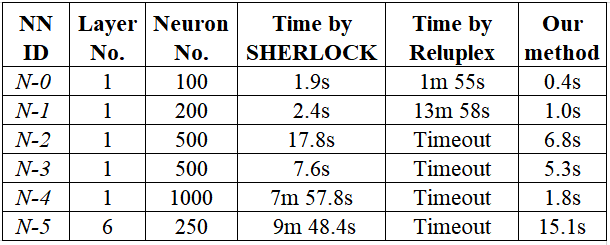
\includegraphics[width=0.9\linewidth]{images/robustnessVerification/f2.png}
% % 	\caption{Comparison with SHERLOCK and Reluplex}
% % 	\label{fig-2}
% % \end{figure}

% % \begin{figure*}[ht]
% % 	\begin{minipage}{0.46\linewidth}
% % 	\centering
% % 	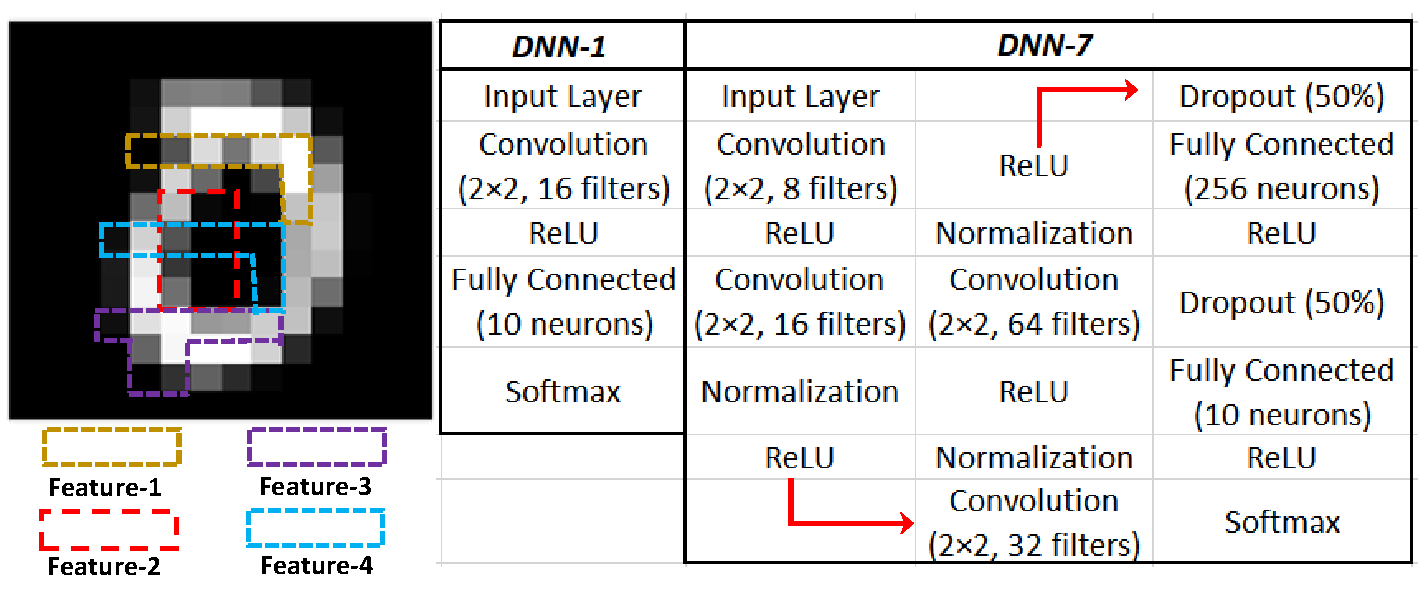
\includegraphics[width=1\linewidth]{images/robustnessVerification/f4.pdf}
% % 	\subcaption{}
% % 		\end{minipage}
% % 		\begin{minipage}{0.54\linewidth}
% % 		\centering
% % 	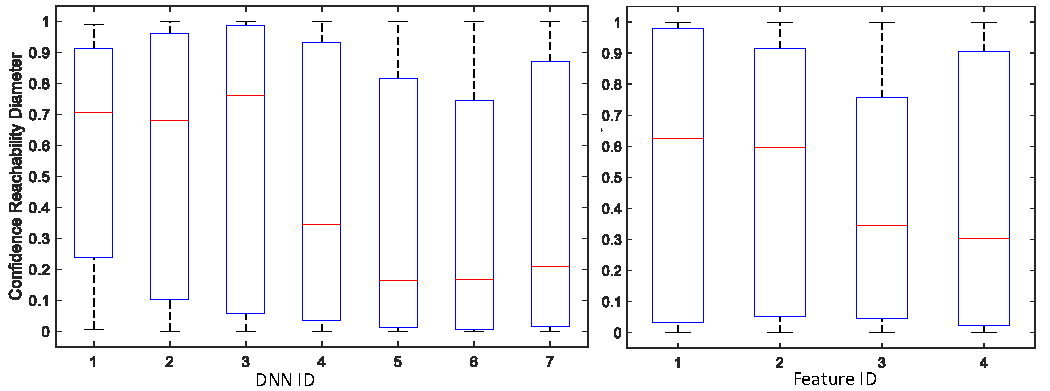
\includegraphics[width=1\linewidth]{images/robustnessVerification/f8.pdf}
% % 		\subcaption{}
% % 		\end{minipage}
% % 			\vspace{-1pt}
% % 			\caption{(a) The four features and the architecture of DNN-1 and DNN-7. (b) Left: boxplots of confidence reachability diameters for 7 DNNs, based on $4\times20$ analyses of each DNN. Right: boxplot of confidence reachability diameters for 4 features, based on $7\times20$ analyses of each feature. The red line represents the median value: a lower value indicates a more robust model or feature.}
% % 	\label{fig-3}
% % \end{figure*}

% % \begin{figure*}[t]
% % 	\begin{minipage}{0.32\linewidth}
% % 	\centering
% % 	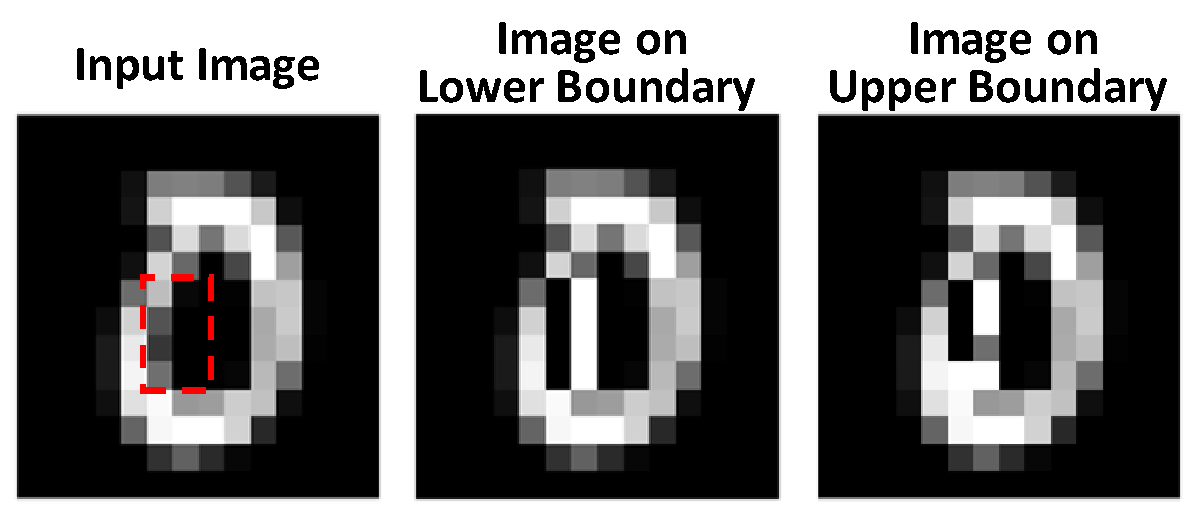
\includegraphics[width=0.9\linewidth]{images/robustnessVerification/f3.pdf}
% % 		\subcaption{}
% % 	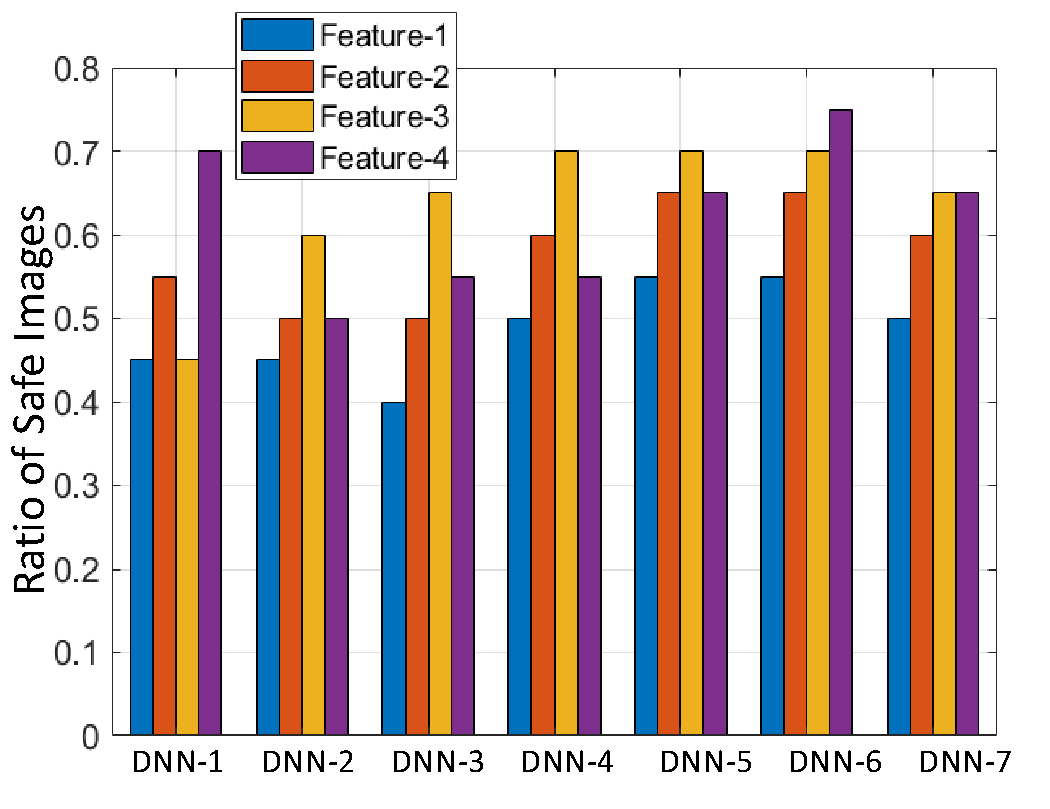
\includegraphics[width=1\linewidth]{images/robustnessVerification/f6.pdf}
% % 	\subcaption{}
% % 		\end{minipage}
% % 		\begin{minipage}{0.68\linewidth}
% % 		\centering
% % 	\centering
% % 	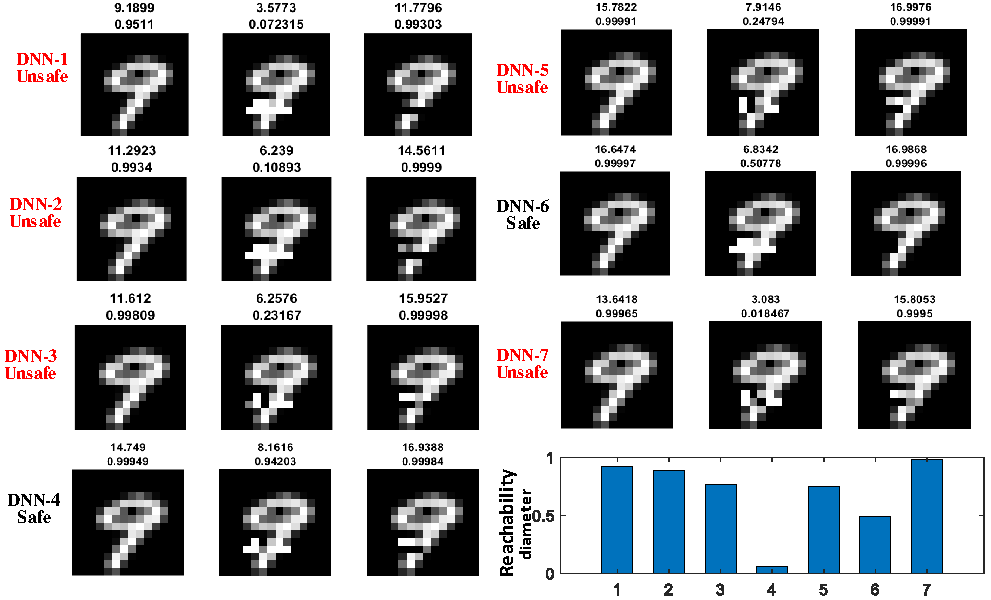
\includegraphics[width=1\linewidth]{images/robustnessVerification/f7.pdf}
% % 	\subcaption{}
% % 		\end{minipage}
% % 			\caption{(a) Left: an original image (logit is 11.806, confidence of output being `0' is 99.95\%), where area marked by dashed line is the feature. Middle: an image on the confidence lower bound. Right: an image on the confidence upper bound; for the output label `0', the feature's output range is $[74.36\%,99.98\%]$, and logit reachability is $[7.007, 13.403]$. (b) Ratios of safe images for 7 DNNs and 4 features. (c) A detailed example comparing the safety and robustness of DNNs for image '9' and Feature-3: the top number in the caption of each figure is logit and the bottom one is confidence; the unsafe cases are all misclassified as `8'; the last bar chart shows their confidence reachability diameters.}
% % 	\label{fig-4}
% % \end{figure*}
 

% % \subsection{Case Study One: Safety Verification}

% % We use our tool to conduct logit and output range analysis.
% % %for verifying the safety of deep neural networks, and compare robustness of different networks and input subspaces. 
% % Seven convolutional neural networks, represented as DNN-1,...,DNN-7, were trained on the MNIST dataset. Images are resized into $14\times 14$ to enforce that a DNN with deeper layers tends to over-fit. The networks have different layer types, including ReLu, dropout and normalization, and the number of layers ranges from $5$ to $19$. Testing accuracies range from $95\%$ to $99\%$, and $\epsilon=0.05$ is used in our experiments.

% % We randomly choose 20 images (2 images per label) and manually choose 4 features
% % %\footnote{We also conduct experiments in which features are selected by object detection techniques such as SIFT \cite{Lowe1999}. We cannot include the results for space limit, but the conclusions are similar. } 
% % such that each feature contains 8 pixels, i.e., $X'=[0,1]^8$. Fig.~\ref{fig-3} (a) illustrates the four features and the architecture of two DNNs with the shallowest and deepest layers, \ie~DNN-1 and DNN-7. 

% % \vspace{1mm}

% % \noindent{\bf Safety Verification}
% % %
% % %Then we conduct the reachability analysis for those features. 
% % Fig.~\ref{fig-4} (a) shows an example: for DNN-1, Feature-4 is \emph{guaranteed to be safe} with respect to the image $x$ and the input subspace $X'$.
% % %to any adversarial perturbation. 
% % Specifically, the reachability interval is $R(\Pi_0,X',\epsilon) = [74.36\%,99.98\%]$, which means that $l(\Pi_0,X',\epsilon)=74.36\%$. By this, we have $u(\oplus_{-0},X',\epsilon) \leq (1-0.7436) < 0.7436 = l(\Pi_0,X',\epsilon)$. Then, by Theorem \ref{thm:safety}, we have 
% % $\Safe(\text{DNN-1},x,X')$. Intuitively, no matter how we manipulate this feature, the worst case is to reduce the confidence of output being `0' from 99.95\% (its original confidence probability) to 74.36\%. 


% % \subsection{Case Study Two: Statistical Quantification of Robustness}


% % \noindent{\bf Statistical Comparison of Safety}
% % %
% % Fig.~\ref{fig-4} (b) compares the ratios of safe images for different DNNs and features. It shows that: \one~no DNN is 100\% safe on those features: DNN-6 is the safest one and DNN-1, DNN-2 and DNN-3 are less safe, which means a DNN with well chosen layers are safer than those DNNs with very shallow or deeper layers; and \two~the safety performance of different DNNs is consistent for the same feature, which suggests that the feature matters -- some features are easily perturbed to yield adversarial examples, e.g., Feature-1 and Feature-2.

% % \vspace{1mm}

% % \noindent{\bf Statistical Comparison of Robustness}
% % %
% % Fig.~\ref{fig-3} (b) compares the robustness of networks and features with two boxplots over the reachability diameters, where the function $o$ is $\Pi_j$ for a suitable $j$. We can see that DNN-6 and DNN-5 are the two most robust, while DNN-1, DNN-2 and DNN-3 are less robust. Moreover, Feature-1 and Feature-2 are less robust than Feature-3 and Feature-4. 

% % %Together with the above, we can see that 
% % We have thus demonstrated that
% % reachability analysis with our tool can be used to quantify the safety and robustness of deep learning models. In the following, we perform a comparison of networks over a fixed feature. 

% % \vspace{1mm}

% \section{A Running Numerical Example}

% In this section, we will use an example to illustrate the fundamental differences of DeepAgn with constraint-solver based approaches and $AI^2$ which is a safety certification method using Abstract Interpretation (AI).

% Fig.~\ref{fig-E2} shows the details of a neural network we used for investigation. This toy neural network has two input $x_1$ and $x_2$, two output $y_1$ and $y_2$. It contains one hidden layer with ReLU activation functions. We denote the ReLU activation by two parts: one part is $r_1$ and $r_1$ denoting the values before the activation, another part is $h_1$ and $h_2$ representing the values after activation. 

% In this case study, we aim to solve the following reachability problem.

% \begin{problem}\label{problem-E1}
% Given a neural network and the box-constraints on its inputs, i.e., $x_1\in [4,6], x_2 \in [4.5,5]$, what is the output range of $y_1$?
% \end{problem}

% We will first show constraint-solver based solution, then reveal how $AI^2$ works and finally show how to use DeepGO to solve this problem.
 
% \begin{figure}[t]
% 	\centering
% 	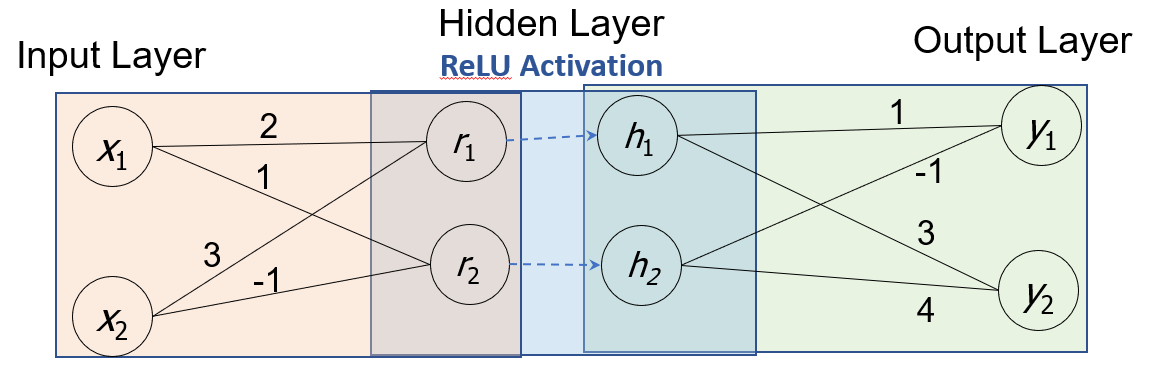
\includegraphics[width=0.85\linewidth]{images/robustnessVerification/Capture5.PNG}
% 	\caption{Encoding the whole neural network layer by layer on a neural networks with one ReLU-based hidden layer}
% 	\label{fig-E2}
% \end{figure}
  
% \subsection{Constraint-Solver based Approaches}

% As shown in Fig.~30, most of the state-of-the-art works on reachability analysis of DNNs are based on MILP or LP solvers, including SHERLOCK~\cite{dutta2017output}, Reluplex~\cite{katz2017reluplex}, Planet~\cite{ehlers2017formal}, MIP~\cite{CNR2017,akintunde2018reachability} and BaB~\cite{bunel2017piecewise}. We will reveal the basic idea of those research works.

% The first step is to encode the input and neural networks. As shown in Fig.~\ref{fig-E2}, we can encode the whole neural network layer by layer.

% \begin{equation}\label{eqn-encode}
%     \begin{split}
%         \begin{cases}
%         r_1 = 2x_1 + 3x_2\\
%         r_2 = x_1 - x_2\\
%         h_1 = \begin{cases}
%     r_1, & \text{if $r_1\geq 0$}.\\
%     0, & \text{otherwise}.
%   \end{cases}\\
%   h_2 = \begin{cases}
%     r_2, & \text{if $r_2\geq 0$}.\\
%     0, & \text{otherwise}.
%   \end{cases}\\
%   y_1 = h_1 - h_2\\
%   y_2 = 3h_1 - 4h_2\\
%   4 \leq x_1 \leq 6\\
%   4.5 \leq x_2 \leq 5
%   \end{cases}
%     \end{split}
% \end{equation}

% Then, to estimate the reachable interval of $y_1$, we also need to incorporate the target problem and formulate them into four linear programming problems based on the activation patterns of hidden neurons, as shown by the below equation.

% \begin{equation}\label{eqn-encode}
%     \begin{split}
%       & \begin{cases}
%         \max/\min~~y_1 = x_1 +4x_2\\
%         \text{s.t.} \quad  2x_1 + 3x_2\geq 0\\
%         \qquad x_1 - x_2 \geq 0\\
%         \qquad 4\leq x_1 \leq 6\\
%         \qquad 4.5\leq x_1 \leq 5\\
%   \end{cases} 
%   \bigcup  
%         \begin{cases}
%         \max/\min~~y_1 = 2x_1 +3x_2\\
%         \text{s.t.} \quad  2x_1 + 3x_2\geq 0\\
%         \qquad x_1 - x_2 \leq 0\\
%         \qquad 4\leq x_1 \leq 6\\
%         \qquad 4.5\leq x_1 \leq 5\\
%   \end{cases}\\
%   \bigcup &
%   \begin{cases}
%         \max/\min~~y_1 = -x_1 +x_2\\
%         \text{s.t.} \quad  2x_1 + 3x_2\leq 0\\
%         \qquad x_1 - x_2 \geq 0\\
%         \qquad 4\leq x_1 \leq 6\\
%         \qquad 4.5\leq x_1 \leq 5\\
%   \end{cases}
%     \bigcup
%   \begin{cases}
%         \max/\min~~y_1 = 0\\
%         \text{s.t.} \quad  2x_1 + 3x_2\leq 0\\
%         \qquad x_1 - x_2 \leq 0\\
%         \qquad 4\leq x_1 \leq 6\\
%         \qquad 4.5\leq x_1 \leq 5\\
%   \end{cases}
%     \end{split}
% \end{equation}

% By solving the above four linear programming problems using some LP solvers, we can solve Problem~\ref{problem-E1} and get its reachable confidence interval $[21.5, 26]$.


% \begin{figure}[t]
% 	\centering
% 	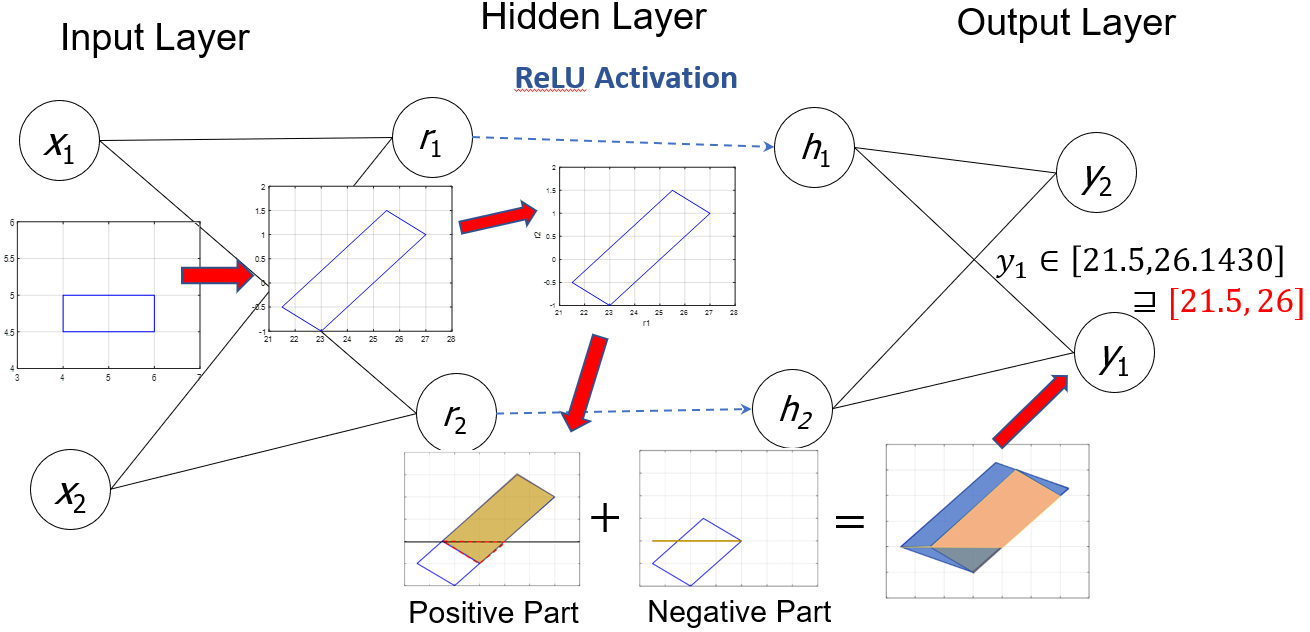
\includegraphics[width=1\linewidth]{images/robustnessVerification/Capture8.PNG}
% 	\caption{Illustration of layer-by-layer over-approximation using zonotope abstract interpretation in $AI^2$}
% 	\label{fig-E11}
% \end{figure}

% \subsubsection{Abstract Interpretation based Approach}

% The most notable safety verification work using Abstract Interpretation is $AI^2$~\cite{gehr2018ai2}. It phrases the problem of analyzing neural networks in the classic framework of abstract interpretation. The key ingredient in $AI^2$ is the layer-by-layer over-approximation in deep neural networks using zonohydron-based abstract interpretation. 

% Figure~\ref{fig-E11} depicts the procedure of layer-by-layer zonotope abstract interpretation in $AI^2$ for solving Problem~\ref{problem-E1}. $AI^2$ first adopts a zonotope to abstract all the inputs. 
% %
% \begin{equation}
%     \begin{split}
%         Z_1 = \{(x_1,x_2)~|~x_1 = a_1 +5; x_2= 0.25a_2 +4.75\}
%     \end{split}
% \end{equation}
% %
% where $a_1 \in [-1,1]$ and $a_2 \in [-1,1]$.

% Then it performs the zonotope abstract transformation based on the affine transformation from input layer into the pre-activation layer. Please note that affine transformation is exact in zonotope-based abstraction.
% %
% \begin{equation}
%     \begin{split}
%         Z_2 = \{(r_1,r_2)~|~r_1 = 24.25+2a_1+0.75a_2; r_2= 0.25 + a_1 - 0.25a_2\}
%     \end{split}
% \end{equation}
% %
% where $a_1 \in [-1,1]$ and $a_2 \in [-1,1]$.

% Next, $AI^2$ considers the zonotope over-approximation on the first ReLU hidden neuron. Since $r_1\geq 0$ always holds, zonohedron $Z_2$ will transfer into the next layer without over-approximation loss. Thus we have $Z_3 = Z_2$. However, for the second ReLU hidden neuron, the zonotope abstraction is complicated since $r2$ is partially negative and partially positive, which requires two cases:

% \begin{itemize}
%     \item Zonotope Over-approximation on Positive Part: As shown in Figure~\ref{fig-E11}, the positive part $Z_3\cap \{r_2\geq 0\}$ is not a zonohedron. So we perform the zonotope over-approximation and get a new zonohedron:
%     $$Z_{4,p} = \{(h_1,h_2)~|~h_1 = 24.75+1.5a_1+0.75a_2; h_2= 0.5 + 0.75a_1 - 0.25a_2\}$$
    
%      \item Zonotope Over-approximation on Negative Part: Similarly, we get a new zonotope 
%     $$Z_{4,n} = \{(h_1,h_2)~|~h_1 = 23.25+0.75a_1+a_2; r_2 = 0\}$$
% \end{itemize}

% Then, as shown in Figure~\ref{fig-E11}, we perform a joint on two zonotopes $Z_{4,p}\cup Z_{4,n}$, and peform another zonotope over-approximation:
% %
% \begin{equation}
%     Z_5 = \{(h_1,h_2)~|~h_1 = 24.3929+1.6429a_1+1.25a_2; h_2= 0.5714 + 0.8214a_1 - 0.25a_2\}
% \end{equation}
% %
% where $a_1 \in [-1,1]$ and $a_2 \in [-1,1]$.

% \begin{figure}[t]
% 	\centering
% 	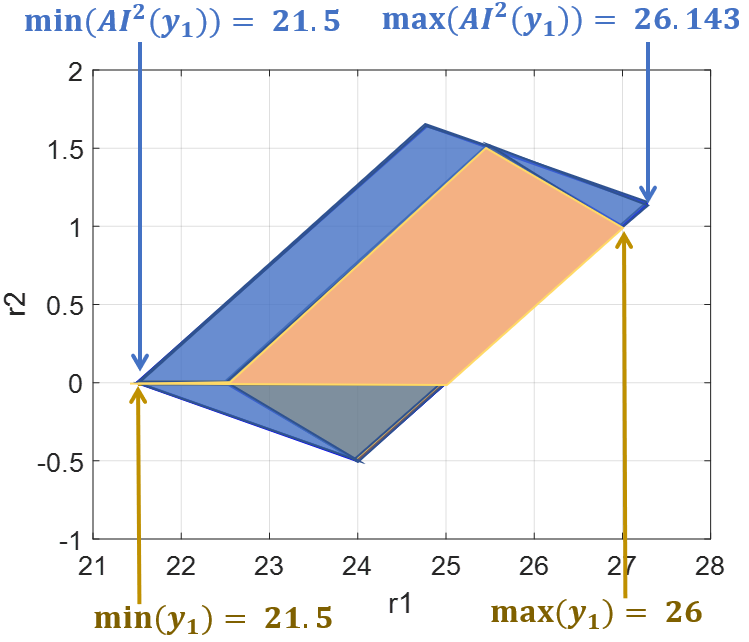
\includegraphics[width=0.55\linewidth]{images/robustnessVerification/Capture9.PNG}
% 	\caption{The comparison between $AI^2$ and DeepAGN in terms of over-approximation loss}
% 	\label{fig-E12}
% \end{figure}

% Finally, we can get the symbolic express on $y_1$ based on the affine transformation from after-activation layer to output layer:
% \begin{equation}
%     y_1 = h1 - h2 = 23.8215 + 0.8215a_1 - 1.5a_2
% \end{equation}
% where $a_1 \in [-1,1]$ and $a_2 \in [-1,1]$. Thus, using $AI^2$, we can get the reachable output of $y_1$ is $[21.5, 26.1430] \supseteq	[21.5, 26]$, which is an over-approximation of the actual reachable state of the neural network. As illustrated by Figure~\ref{fig-E12}, the yellow area is the actually information passed into the output layer and the blue area is the over-approximation loss brought by the layer-by-layer zonotope abstractions.

% \begin{figure}[t]
% 	\centering
% 	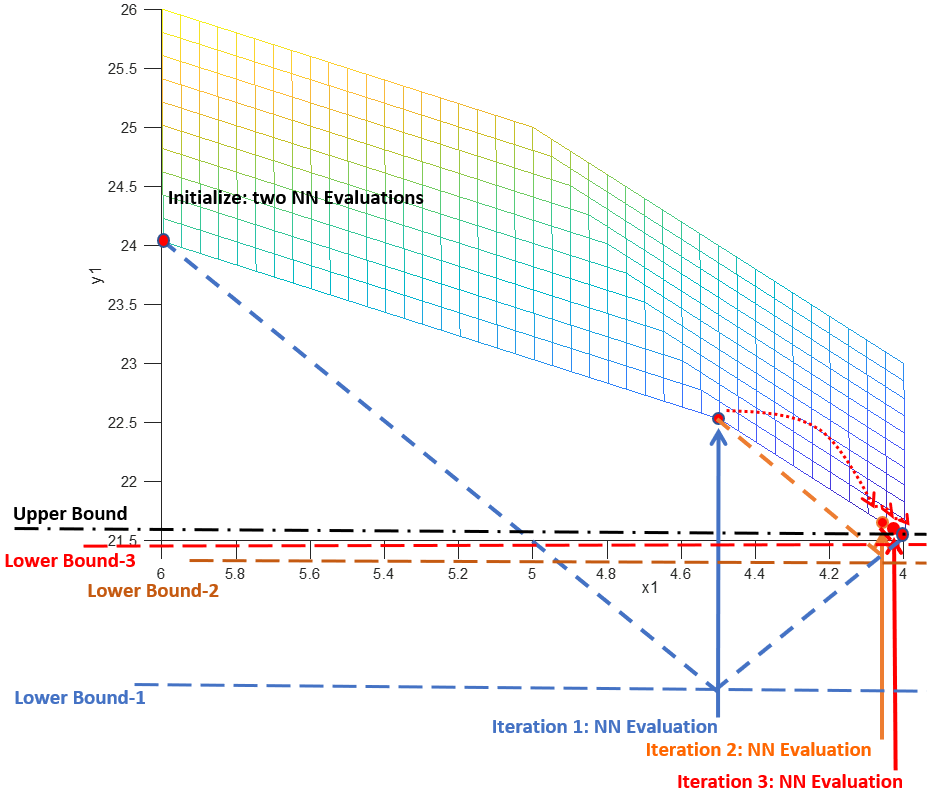
\includegraphics[width=0.9\linewidth]{images/robustnessVerification/Capture10.PNG}
% 	\caption{Illustration of working mechanism of DeepGO for solving the reachability problem}
% 	\label{fig-E13}
% \end{figure}

% % In this section, we show the experimental evidence for the utility of our algorithm. Our method is implemented in Python 3.7, running on a computer with i7-4770 CPU, 24GB RAM and NVIDIA Quadro P5000 GPU. The experiments consist of two parts. In the first part we demonstrate that our method outperforms these existed methods in accuracy. In the second part we show various application scenarios of our verification method, which are speech recognition and handwriting recognition with CRNN respectively. These implementations also prove the  applicability of our method on different recurrent networks, as long as the network is Lipschitz continuous. We verify the safety and robustness of RNNs by conducting the output range analysis of the whole input range. Moreover, when the RNN is not safe in the whole input range, our method can calculate the maximal safe radius and concrete the ground-truth adversarial example.

% \subsection{Reachability Analysis by Lipschitz Optimisation}


% This section will show how DeepGO works. Since the neural network is Lipschitz continuous (as proved in Section 3), to solve Problem~\ref{problem-E1}, it can be reduces to solve the following minimization problems.
% \begin{equation}\label{eqn-deepagn}
%   \begin{cases}
%         \min_{x_1,x_2}~~y_1 = f(x_1,x_2)\\
%         \text{s.t.} \quad 4\leq x_1 \leq 6\\
%         \qquad 4.5\leq x_1 \leq 5\\
%   \end{cases}
% \end{equation}

% By solving the above two problems, we can get the reachable value of $y_1$. Figure~\ref{fig-E13} illustrates the optimization procedure of DeepAgn iteration by iteration\footnote{For visualization, we just show the $x_1$ dimension.}.

% \begin{itemize}
%     \item Initialization: It evaluates two ending points on $x_1$: 4 and 6, and get the Upper Bound and Lower Bound-1.
%     \item Iterations: DeepAgn then evaluates $y_1$ on the point of Lower Bound-1, and refine the lower bound to get Lower Bound-2 (descriped in Section 6.1). Similarly, we continues the optimization iterations and get a series of lower bounds.
%     \item Termination: After the gap between lower bound and upper bound is close enough, i.e., smaller than an positive number $\epsilon = 0.0001$, we stop and return the value of $y_1^* = 21.5$, which is the lowest value that the neural network can reach in Problem~\ref{problem-E1}.
% \end{itemize}
% \begin{algorithm}[ht]  
%     \caption{Calculation of maximal safe radius for target attack}
%     \label{alg:alg1}
%     \begin{algorithmic}[1]
%     \REQUIRE $f$, $x_0$, $\theta_0$, $\epsilon$, original label $j$, target label $k$, $a$, $b$
%     \ENSURE maximal safe radius $r$ 
%     \STATE $\theta \leftarrow \theta_0, \theta_{min} \leftarrow 0,\theta_{max} \leftarrow (b-a) $
%         \FOR{$i$ in range $N$}
%             \STATE $l_j,x_j \leftarrow DeepAgnmin(f,x_0,x',\theta,a,b,j)$ 
% 	        \STATE $u_k,x_k \leftarrow DeepAgnmax(f,x_0,x',\theta,a,b,k)$ 
%             \STATE {$i++$}
% 		    \IF{$l_j-u_k > \epsilon$} 
% 		        \STATE $\theta \leftarrow (\theta + \theta_{max})/2 $ 
% 		    \ELSIF{$u_k-l_j > \epsilon$} 
% 			    \STATE $\theta \leftarrow (\theta + \theta_{min})/2$ 
% 		    \ELSE
% 		        \STATE break
% 		    \ENDIF
% 		\ENDFOR
% 	    \STATE $r=\theta$
% 	\end{algorithmic}     
% \end{algorithm}
% To get the largest reachable value, We replace objective function in Eqn.~\ref{eqn-deepagn} by $y_1 = - f(x_1,x_2)$ and perform the same procedure to get $y_1^{**} = 26$. By DeepAgn, we can finally get the reachable interval of the neural network: $y_1 = [21.5, 26]$. Comparing to $AI^2$, DeepAgn is both sound and complete in an arbitrary precision (controlled by value of $\epsilon$).



% When the network $f$ is not safe with certain perturbation, it means we can find a label $k$ with $u_k\ge{l_j}$. In such case, we reduce the perturbation, i.e. norm ball radius, step by step with binary search until we find the maximal safe norm ball. We add an limitation of perturbation of $\theta$ in the Eqn.~(\ref{optimization}) and %optimization \ref{optimization} and  
% \begin{equation}
% \begin{split}
%      &l= \min{f(\underline{X_0}\cup{X'})}\\
% subject\ to \quad &max(a,x-\theta)\le{x'}\le min(b,x+\theta)
% \end{split}
% \end{equation}


% {Algorithm~\ref{alg:alg1} shows the calculation for the maximal safe radius.}


% \section{Conclusion}

% We propose, design and implement a reachability analysis tool for deep neural networks, which has provable guarantees and can be applied to neural networks with deep layers and nonlinear activation functions. The experiments demonstrate that our tool can be utilized to verify the safety of deep neural networks and quantitatively compare their robustness. We envision that this work marks an important step towards a practical, guaranteed safety verification for DNNs. Future work includes parallelizing this method in GPUs to improve its scalability on large-scale models trained on ImageNet, and a generalisation %of this method to work with 
% to other deep learning models such as RNNs and deep reinforcement learning.
